\documentclass[twoside]{book}

% Packages required by doxygen
\usepackage{fixltx2e}
\usepackage{calc}
\usepackage{doxygen}
\usepackage[export]{adjustbox} % also loads graphicx
\usepackage{graphicx}
\usepackage[utf8]{inputenc}
\usepackage{makeidx}
\usepackage{multicol}
\usepackage{multirow}
\PassOptionsToPackage{warn}{textcomp}
\usepackage{textcomp}
\usepackage[nointegrals]{wasysym}
\usepackage[table]{xcolor}

% Font selection
\usepackage[T1]{fontenc}
\usepackage[scaled=.90]{helvet}
\usepackage{courier}
\usepackage{amssymb}
\usepackage{sectsty}
\renewcommand{\familydefault}{\sfdefault}
\allsectionsfont{%
  \fontseries{bc}\selectfont%
  \color{darkgray}%
}
\renewcommand{\DoxyLabelFont}{%
  \fontseries{bc}\selectfont%
  \color{darkgray}%
}
\newcommand{\+}{\discretionary{\mbox{\scriptsize$\hookleftarrow$}}{}{}}

% Page & text layout
\usepackage{geometry}
\geometry{%
  a4paper,%
  top=2.5cm,%
  bottom=2.5cm,%
  left=2.5cm,%
  right=2.5cm%
}
\tolerance=750
\hfuzz=15pt
\hbadness=750
\setlength{\emergencystretch}{15pt}
\setlength{\parindent}{0cm}
\setlength{\parskip}{3ex plus 2ex minus 2ex}
\makeatletter
\renewcommand{\paragraph}{%
  \@startsection{paragraph}{4}{0ex}{-1.0ex}{1.0ex}{%
    \normalfont\normalsize\bfseries\SS@parafont%
  }%
}
\renewcommand{\subparagraph}{%
  \@startsection{subparagraph}{5}{0ex}{-1.0ex}{1.0ex}{%
    \normalfont\normalsize\bfseries\SS@subparafont%
  }%
}
\makeatother

% Headers & footers
\usepackage{fancyhdr}
\pagestyle{fancyplain}
\fancyhead[LE]{\fancyplain{}{\bfseries\thepage}}
\fancyhead[CE]{\fancyplain{}{}}
\fancyhead[RE]{\fancyplain{}{\bfseries\leftmark}}
\fancyhead[LO]{\fancyplain{}{\bfseries\rightmark}}
\fancyhead[CO]{\fancyplain{}{}}
\fancyhead[RO]{\fancyplain{}{\bfseries\thepage}}
\fancyfoot[LE]{\fancyplain{}{}}
\fancyfoot[CE]{\fancyplain{}{}}
\fancyfoot[RE]{\fancyplain{}{\bfseries\scriptsize Generated by Doxygen }}
\fancyfoot[LO]{\fancyplain{}{\bfseries\scriptsize Generated by Doxygen }}
\fancyfoot[CO]{\fancyplain{}{}}
\fancyfoot[RO]{\fancyplain{}{}}
\renewcommand{\footrulewidth}{0.4pt}
\renewcommand{\chaptermark}[1]{%
  \markboth{#1}{}%
}
\renewcommand{\sectionmark}[1]{%
  \markright{\thesection\ #1}%
}

% Indices & bibliography
\usepackage{natbib}
\usepackage[titles]{tocloft}
\setcounter{tocdepth}{3}
\setcounter{secnumdepth}{5}
\makeindex

% Hyperlinks (required, but should be loaded last)
\usepackage{ifpdf}
\ifpdf
  \usepackage[pdftex,pagebackref=true]{hyperref}
\else
  \usepackage[ps2pdf,pagebackref=true]{hyperref}
\fi
\hypersetup{%
  colorlinks=true,%
  linkcolor=blue,%
  citecolor=blue,%
  unicode%
}

% Custom commands
\newcommand{\clearemptydoublepage}{%
  \newpage{\pagestyle{empty}\cleardoublepage}%
}

\usepackage{caption}
\captionsetup{labelsep=space,justification=centering,font={bf},singlelinecheck=off,skip=4pt,position=top}

%===== C O N T E N T S =====

\begin{document}

% Titlepage & ToC
\hypersetup{pageanchor=false,
             bookmarksnumbered=true,
             pdfencoding=unicode
            }
\pagenumbering{alph}
\begin{titlepage}
\vspace*{7cm}
\begin{center}%
{\Large E\+E\+C\+E435\+L\+\_\+\+Game\+\_\+\+Framework }\\
\vspace*{1cm}
{\large Generated by Doxygen 1.8.13}\\
\end{center}
\end{titlepage}
\clearemptydoublepage
\pagenumbering{roman}
\tableofcontents
\clearemptydoublepage
\pagenumbering{arabic}
\hypersetup{pageanchor=true}

%--- Begin generated contents ---
\chapter{E\+E\+CE 435L Game Framework}
\label{index}\hypertarget{index}{}\begin{DoxyAuthor}{Author}
Karim Zarzour 

Maarouf Yassine 
\end{DoxyAuthor}
\begin{DoxyDate}{Date}
20-\/11-\/2021 
\end{DoxyDate}

\chapter{R\+E\+A\+D\+ME}
\label{md_README}
\Hypertarget{md_README}
This R\+E\+A\+D\+ME would normally document whatever steps are necessary to get your application up and running.

\subsubsection*{What is this repository for?}


\begin{DoxyItemize}
\item Quick summary
\item Version
\item \href{https://bitbucket.org/tutorials/markdowndemo}{\tt Learn Markdown}
\end{DoxyItemize}

\subsubsection*{How do I get set up?}


\begin{DoxyItemize}
\item Summary of set up
\item Configuration
\item Dependencies
\item Database configuration
\item How to run tests
\item Deployment instructions
\end{DoxyItemize}

\subsubsection*{Contribution guidelines}


\begin{DoxyItemize}
\item Writing tests
\item Code review
\item Other guidelines
\end{DoxyItemize}

\subsubsection*{Who do I talk to?}


\begin{DoxyItemize}
\item Repo owner or admin
\item Other community or team contact 
\end{DoxyItemize}
\chapter{Hierarchical Index}
\section{Class Hierarchy}
This inheritance list is sorted roughly, but not completely, alphabetically\+:\begin{DoxyCompactList}
\item \contentsline{section}{Json\+Utils}{\pageref{classJsonUtils}}{}
\item Q\+Graphics\+Pixmap\+Item\begin{DoxyCompactList}
\item \contentsline{section}{Disk}{\pageref{classDisk}}{}
\item \contentsline{section}{Lower\+Panel\+Button}{\pageref{classLowerPanelButton}}{}
\item \contentsline{section}{missed\+Disk\+Zone}{\pageref{classmissedDiskZone}}{}
\end{DoxyCompactList}
\item Q\+Graphics\+Scene\begin{DoxyCompactList}
\item \contentsline{section}{Game1\+Game\+Page}{\pageref{classGame1GamePage}}{}
\item \contentsline{section}{Game1\+Welcome\+Page}{\pageref{classGame1WelcomePage}}{}
\item \contentsline{section}{Game2\+Game\+Page}{\pageref{classGame2GamePage}}{}
\item \contentsline{section}{Game2\+Welcome\+Page}{\pageref{classGame2WelcomePage}}{}
\item \contentsline{section}{main\+Page}{\pageref{classmainPage}}{}
\end{DoxyCompactList}
\item Q\+Graphics\+View\begin{DoxyCompactList}
\item \contentsline{section}{App\+Main\+View}{\pageref{classAppMainView}}{}
\item \contentsline{section}{Game1\+View}{\pageref{classGame1View}}{}
\item \contentsline{section}{Game2\+View}{\pageref{classGame2View}}{}
\end{DoxyCompactList}
\item Q\+Object\begin{DoxyCompactList}
\item \contentsline{section}{Disk}{\pageref{classDisk}}{}
\item \contentsline{section}{Lower\+Panel\+Button}{\pageref{classLowerPanelButton}}{}
\item \contentsline{section}{missed\+Disk\+Zone}{\pageref{classmissedDiskZone}}{}
\item \contentsline{section}{Question\+Obj}{\pageref{classQuestionObj}}{}
\item \contentsline{section}{User}{\pageref{classUser}}{}
\end{DoxyCompactList}
\item Q\+Widget\begin{DoxyCompactList}
\item \contentsline{section}{command\+Panel}{\pageref{classcommandPanel}}{}
\item \contentsline{section}{Landing\+Page}{\pageref{classLandingPage}}{}
\item \contentsline{section}{Question\+Page}{\pageref{classQuestionPage}}{}
\item \contentsline{section}{Signup\+Page}{\pageref{classSignupPage}}{}
\end{DoxyCompactList}
\end{DoxyCompactList}

\chapter{Class Index}
\section{Class List}
Here are the classes, structs, unions and interfaces with brief descriptions\+:\begin{DoxyCompactList}
\item\contentsline{section}{\hyperlink{classAppMainView}{App\+Main\+View} }{\pageref{classAppMainView}}{}
\item\contentsline{section}{\hyperlink{classcommandPanel}{command\+Panel} }{\pageref{classcommandPanel}}{}
\item\contentsline{section}{\hyperlink{classDisk}{Disk} }{\pageref{classDisk}}{}
\item\contentsline{section}{\hyperlink{classGame1GamePage}{Game1\+Game\+Page} }{\pageref{classGame1GamePage}}{}
\item\contentsline{section}{\hyperlink{classGame1View}{Game1\+View} }{\pageref{classGame1View}}{}
\item\contentsline{section}{\hyperlink{classGame1WelcomePage}{Game1\+Welcome\+Page} }{\pageref{classGame1WelcomePage}}{}
\item\contentsline{section}{\hyperlink{classGame2GamePage}{Game2\+Game\+Page} }{\pageref{classGame2GamePage}}{}
\item\contentsline{section}{\hyperlink{classGame2View}{Game2\+View} }{\pageref{classGame2View}}{}
\item\contentsline{section}{\hyperlink{classGame2WelcomePage}{Game2\+Welcome\+Page} }{\pageref{classGame2WelcomePage}}{}
\item\contentsline{section}{\hyperlink{classJsonUtils}{Json\+Utils} }{\pageref{classJsonUtils}}{}
\item\contentsline{section}{\hyperlink{classLandingPage}{Landing\+Page} }{\pageref{classLandingPage}}{}
\item\contentsline{section}{\hyperlink{classLowerPanelButton}{Lower\+Panel\+Button} }{\pageref{classLowerPanelButton}}{}
\item\contentsline{section}{\hyperlink{classmainPage}{main\+Page} }{\pageref{classmainPage}}{}
\item\contentsline{section}{\hyperlink{classmissedDiskZone}{missed\+Disk\+Zone} }{\pageref{classmissedDiskZone}}{}
\item\contentsline{section}{\hyperlink{classQuestionObj}{Question\+Obj} }{\pageref{classQuestionObj}}{}
\item\contentsline{section}{\hyperlink{classQuestionPage}{Question\+Page} }{\pageref{classQuestionPage}}{}
\item\contentsline{section}{\hyperlink{classSignupPage}{Signup\+Page} }{\pageref{classSignupPage}}{}
\item\contentsline{section}{\hyperlink{classUser}{User} }{\pageref{classUser}}{}
\end{DoxyCompactList}

\chapter{Class Documentation}
\hypertarget{classAppMainView}{}\section{App\+Main\+View Class Reference}
\label{classAppMainView}\index{App\+Main\+View@{App\+Main\+View}}


Inheritance diagram for App\+Main\+View\+:\nopagebreak
\begin{figure}[H]
\begin{center}
\leavevmode
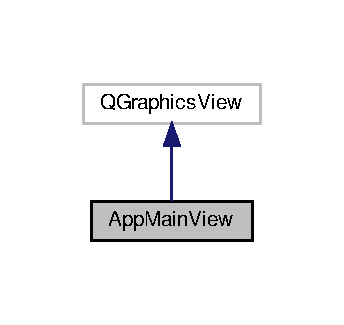
\includegraphics[width=165pt]{classAppMainView__inherit__graph}
\end{center}
\end{figure}


Collaboration diagram for App\+Main\+View\+:
\nopagebreak
\begin{figure}[H]
\begin{center}
\leavevmode
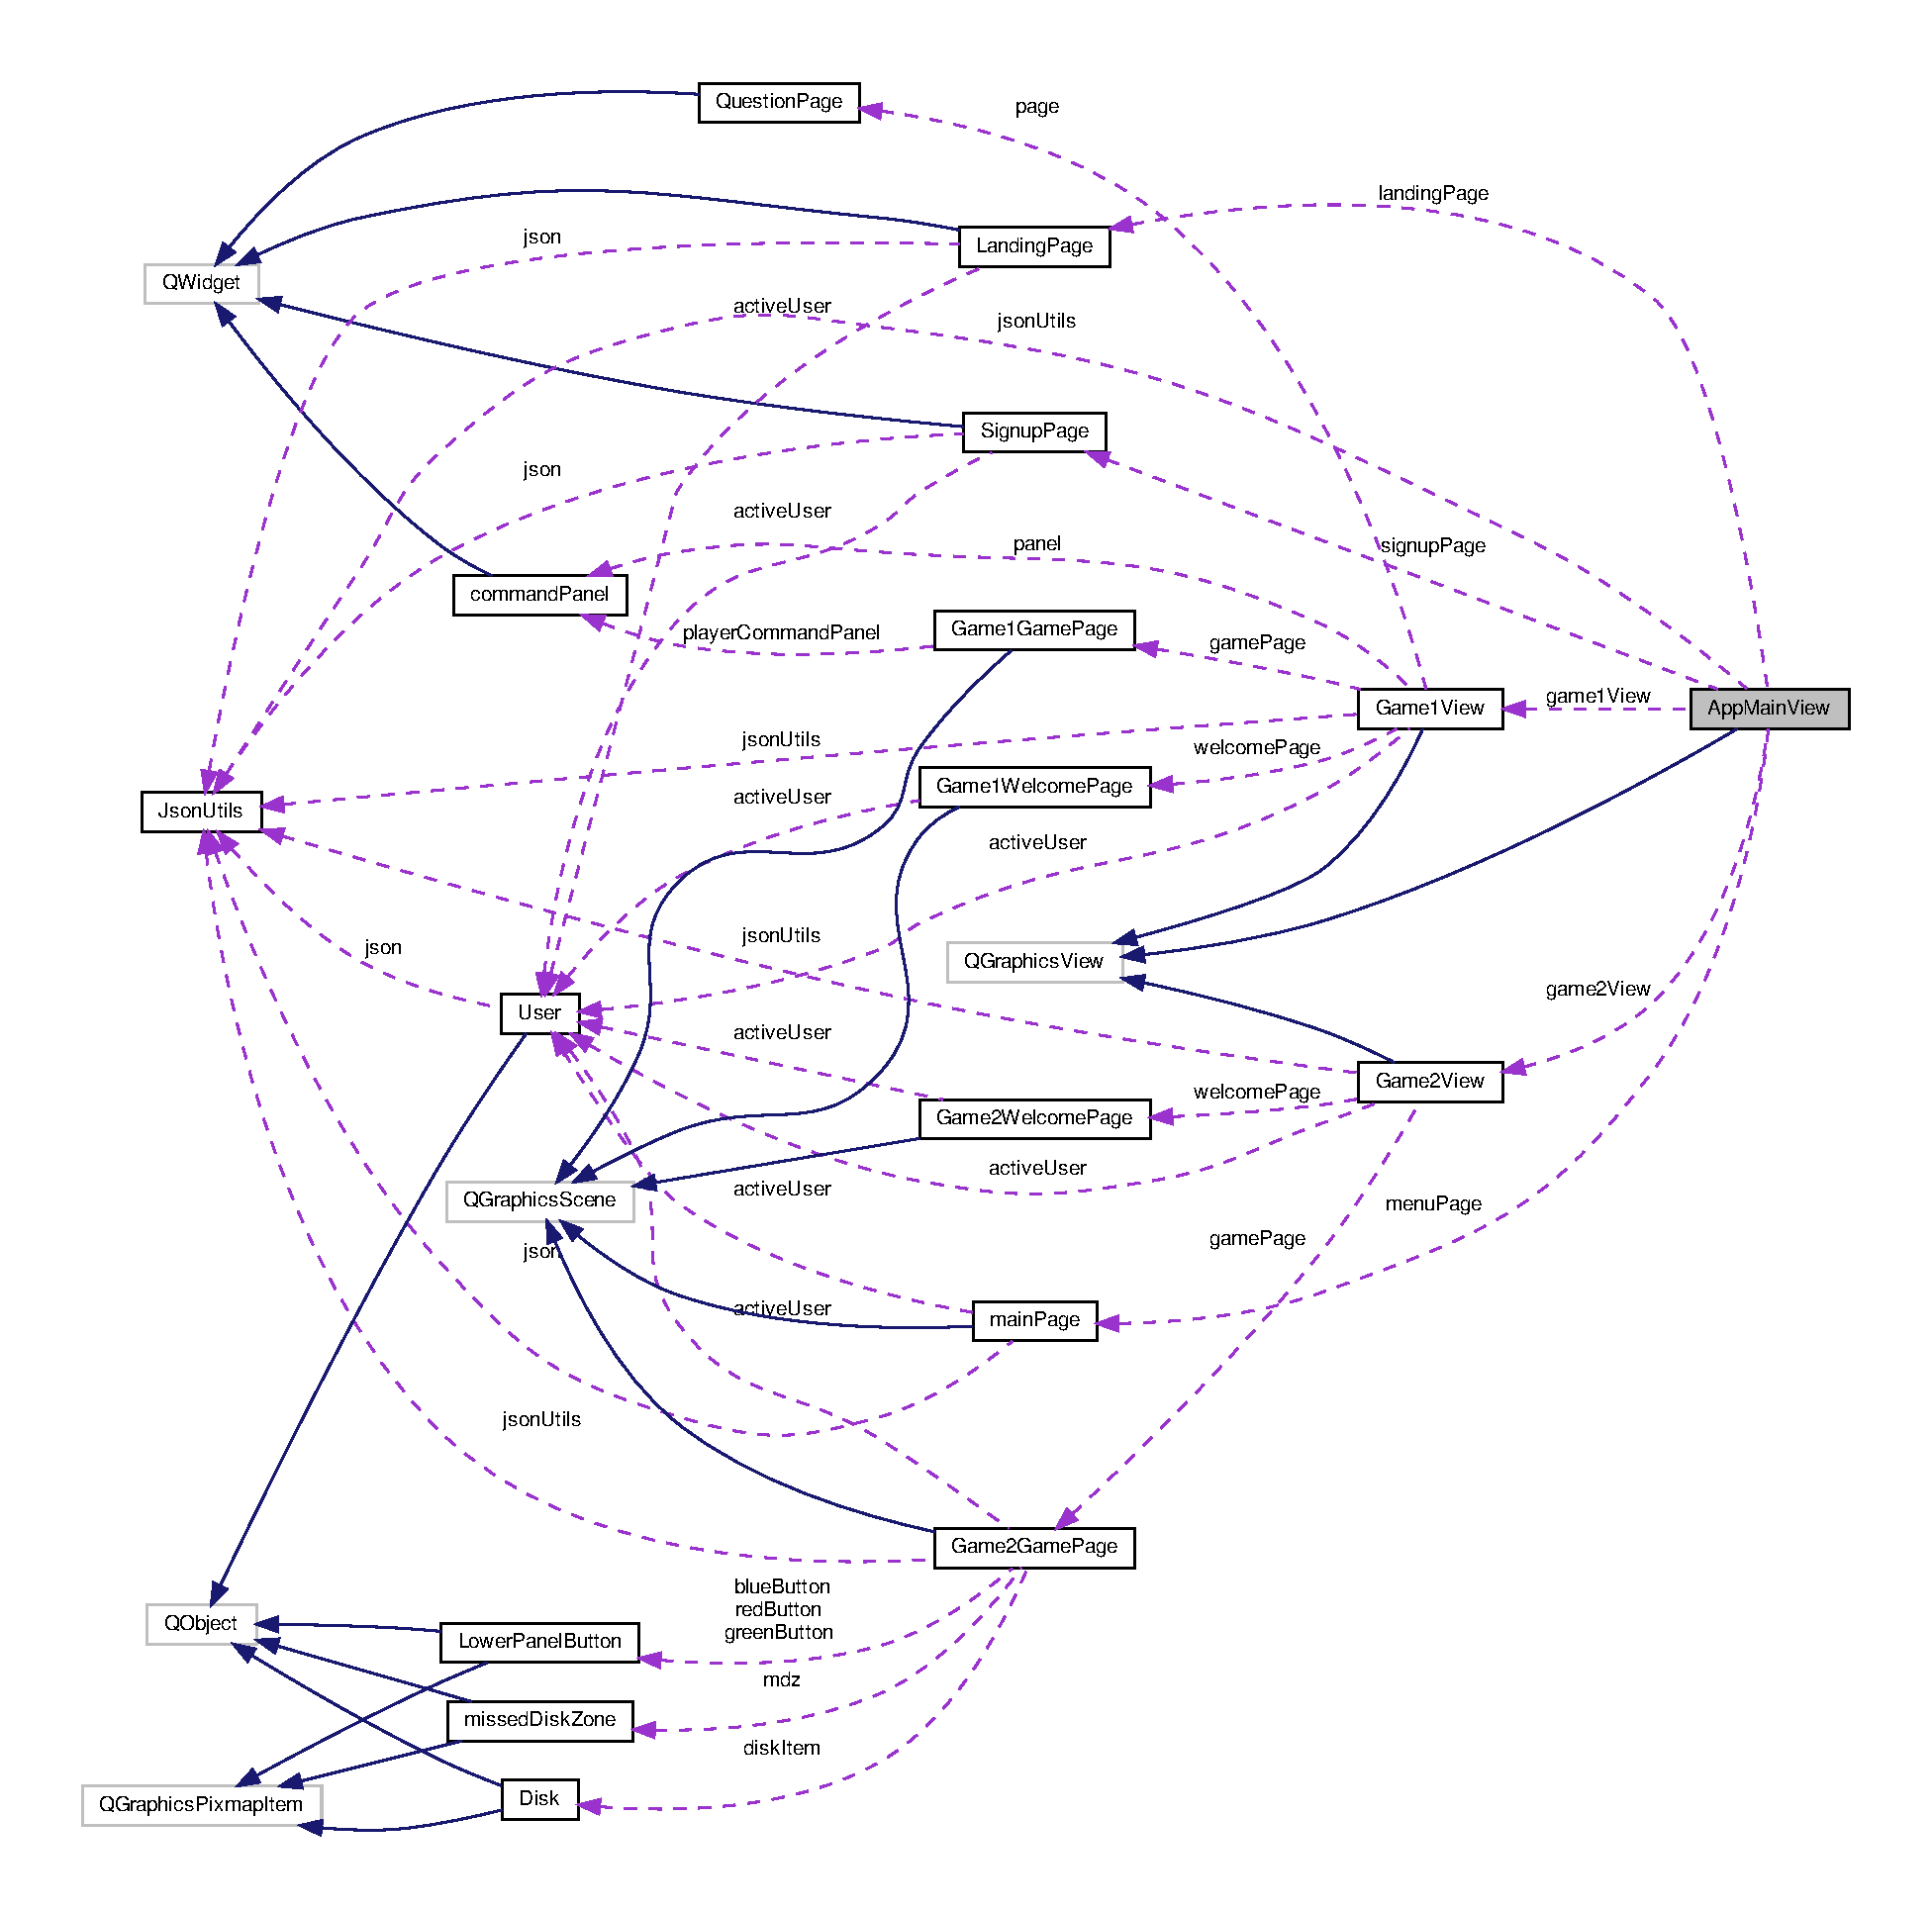
\includegraphics[width=350pt]{classAppMainView__coll__graph}
\end{center}
\end{figure}
\subsection*{Public Slots}
\begin{DoxyCompactItemize}
\item 
\mbox{\Hypertarget{classAppMainView_a4b957db57f6eb234151b7569d7290a43}\label{classAppMainView_a4b957db57f6eb234151b7569d7290a43}} 
void \hyperlink{classAppMainView_a4b957db57f6eb234151b7569d7290a43}{signup} ()
\begin{DoxyCompactList}\small\item\em \hyperlink{classAppMainView_a4b957db57f6eb234151b7569d7290a43}{App\+Main\+View\+::signup}, changes the page to the signup page. \end{DoxyCompactList}\item 
\mbox{\Hypertarget{classAppMainView_ac195b1ff1ef242180c9adf634f39ea1f}\label{classAppMainView_ac195b1ff1ef242180c9adf634f39ea1f}} 
void \hyperlink{classAppMainView_ac195b1ff1ef242180c9adf634f39ea1f}{open\+Main\+Page} ()
\begin{DoxyCompactList}\small\item\em \hyperlink{classAppMainView_ac195b1ff1ef242180c9adf634f39ea1f}{App\+Main\+View\+::open\+Main\+Page}, changes the page to the main page. \end{DoxyCompactList}\item 
\mbox{\Hypertarget{classAppMainView_a13520db5cb1b50330e79b71d14563a05}\label{classAppMainView_a13520db5cb1b50330e79b71d14563a05}} 
void \hyperlink{classAppMainView_a13520db5cb1b50330e79b71d14563a05}{play\+As\+Guest} ()
\begin{DoxyCompactList}\small\item\em \hyperlink{classAppMainView_a13520db5cb1b50330e79b71d14563a05}{App\+Main\+View\+::play\+As\+Guest}, changes the page to the main page and allows player to play without an account. \end{DoxyCompactList}\item 
\mbox{\Hypertarget{classAppMainView_adbde7b357c0307752ff7f1ddf7f28676}\label{classAppMainView_adbde7b357c0307752ff7f1ddf7f28676}} 
void \hyperlink{classAppMainView_adbde7b357c0307752ff7f1ddf7f28676}{login} ()
\begin{DoxyCompactList}\small\item\em \hyperlink{classAppMainView_adbde7b357c0307752ff7f1ddf7f28676}{App\+Main\+View\+::login}, changes the page to the login page and clears widgets. \end{DoxyCompactList}\item 
\mbox{\Hypertarget{classAppMainView_abea602fb374e111e5e14007a96e651e8}\label{classAppMainView_abea602fb374e111e5e14007a96e651e8}} 
void \hyperlink{classAppMainView_abea602fb374e111e5e14007a96e651e8}{authenticate\+User} ()
\begin{DoxyCompactList}\small\item\em \hyperlink{classAppMainView_abea602fb374e111e5e14007a96e651e8}{App\+Main\+View\+::authenticate\+User}, on login checks if the username and password pair are correct. \end{DoxyCompactList}\item 
\mbox{\Hypertarget{classAppMainView_aba3b2431f4395525e73ef0314b16c8ff}\label{classAppMainView_aba3b2431f4395525e73ef0314b16c8ff}} 
void \hyperlink{classAppMainView_aba3b2431f4395525e73ef0314b16c8ff}{log\+Out} ()
\begin{DoxyCompactList}\small\item\em \hyperlink{classAppMainView_aba3b2431f4395525e73ef0314b16c8ff}{App\+Main\+View\+::log\+Out}, logs out the user from their account. \end{DoxyCompactList}\item 
\mbox{\Hypertarget{classAppMainView_ab08130551b14f168d2b927872b3530f4}\label{classAppMainView_ab08130551b14f168d2b927872b3530f4}} 
void \hyperlink{classAppMainView_ab08130551b14f168d2b927872b3530f4}{play\+Game1} ()
\begin{DoxyCompactList}\small\item\em \hyperlink{classAppMainView_ab08130551b14f168d2b927872b3530f4}{App\+Main\+View\+::play\+Game1}, changes page to game 1 welcome page. \end{DoxyCompactList}\item 
\mbox{\Hypertarget{classAppMainView_ae73887df8b33fe982ff9daa0a5449358}\label{classAppMainView_ae73887df8b33fe982ff9daa0a5449358}} 
void \hyperlink{classAppMainView_ae73887df8b33fe982ff9daa0a5449358}{play\+Game2} ()
\begin{DoxyCompactList}\small\item\em \hyperlink{classAppMainView_ae73887df8b33fe982ff9daa0a5449358}{App\+Main\+View\+::play\+Game2}, changes page to game 2 welcome page. \end{DoxyCompactList}\end{DoxyCompactItemize}
\subsection*{Public Member Functions}
\begin{DoxyCompactItemize}
\item 
\mbox{\Hypertarget{classAppMainView_af0d3cdcecdf8f7b717cce0f9803d85c9}\label{classAppMainView_af0d3cdcecdf8f7b717cce0f9803d85c9}} 
void \hyperlink{classAppMainView_af0d3cdcecdf8f7b717cce0f9803d85c9}{connect\+Buttons} ()
\begin{DoxyCompactList}\small\item\em \hyperlink{classAppMainView_af0d3cdcecdf8f7b717cce0f9803d85c9}{App\+Main\+View\+::connect\+Buttons}, connects the buttons to the functions that need to be called when they are clicked. \end{DoxyCompactList}\end{DoxyCompactItemize}
\subsection*{Public Attributes}
\begin{DoxyCompactItemize}
\item 
\mbox{\Hypertarget{classAppMainView_ac1993e81b1591959c70fd0dc81ae7675}\label{classAppMainView_ac1993e81b1591959c70fd0dc81ae7675}} 
\hyperlink{classJsonUtils}{Json\+Utils} $\ast$ {\bfseries json\+Utils}
\item 
\mbox{\Hypertarget{classAppMainView_a6ce48659229761f90082abce3624301e}\label{classAppMainView_a6ce48659229761f90082abce3624301e}} 
\hyperlink{classSignupPage}{Signup\+Page} $\ast$ {\bfseries signup\+Page}
\item 
\mbox{\Hypertarget{classAppMainView_aca2fb901b55b7607addf5fa0a9bcb762}\label{classAppMainView_aca2fb901b55b7607addf5fa0a9bcb762}} 
\hyperlink{classLandingPage}{Landing\+Page} $\ast$ {\bfseries landing\+Page}
\item 
\mbox{\Hypertarget{classAppMainView_a8faef724c48bae43fbe87a9c336ecc8c}\label{classAppMainView_a8faef724c48bae43fbe87a9c336ecc8c}} 
\hyperlink{classmainPage}{main\+Page} $\ast$ {\bfseries menu\+Page}
\item 
\mbox{\Hypertarget{classAppMainView_a57ebafcae52a96567d28734e5bec1298}\label{classAppMainView_a57ebafcae52a96567d28734e5bec1298}} 
\hyperlink{classGame1View}{Game1\+View} $\ast$ {\bfseries game1\+View}
\item 
\mbox{\Hypertarget{classAppMainView_a9380c2ae4d16787838c5819e304d390a}\label{classAppMainView_a9380c2ae4d16787838c5819e304d390a}} 
\hyperlink{classGame2View}{Game2\+View} $\ast$ {\bfseries game2\+View}
\end{DoxyCompactItemize}


The documentation for this class was generated from the following files\+:\begin{DoxyCompactItemize}
\item 
appmainview.\+h\item 
appmainview.\+cpp\end{DoxyCompactItemize}

\hypertarget{classcommandPanel}{}\section{command\+Panel Class Reference}
\label{classcommandPanel}\index{command\+Panel@{command\+Panel}}


Inheritance diagram for command\+Panel\+:
\nopagebreak
\begin{figure}[H]
\begin{center}
\leavevmode
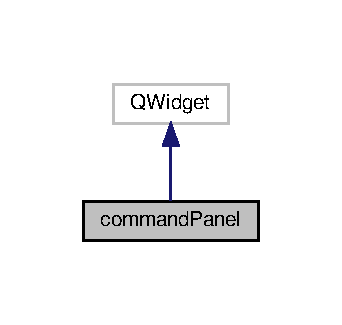
\includegraphics[width=164pt]{classcommandPanel__inherit__graph}
\end{center}
\end{figure}


Collaboration diagram for command\+Panel\+:
\nopagebreak
\begin{figure}[H]
\begin{center}
\leavevmode
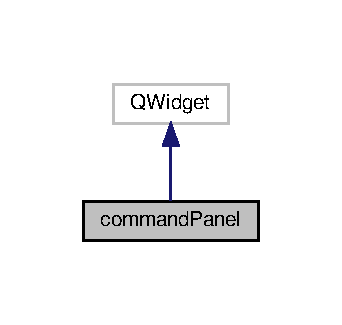
\includegraphics[width=164pt]{classcommandPanel__coll__graph}
\end{center}
\end{figure}
\subsection*{Public Member Functions}
\begin{DoxyCompactItemize}
\item 
\mbox{\Hypertarget{classcommandPanel_a4d5746d112c177124eddf5a5deb00e2f}\label{classcommandPanel_a4d5746d112c177124eddf5a5deb00e2f}} 
{\bfseries command\+Panel} (Q\+Widget $\ast$parent=nullptr)
\end{DoxyCompactItemize}
\subsection*{Public Attributes}
\begin{DoxyCompactItemize}
\item 
\mbox{\Hypertarget{classcommandPanel_ae1efb014f348de12388614e3b6300863}\label{classcommandPanel_ae1efb014f348de12388614e3b6300863}} 
Q\+Label $\ast$ {\bfseries main\+Label}
\item 
\mbox{\Hypertarget{classcommandPanel_ad3af6fe471db6a90d28c1068ce297612}\label{classcommandPanel_ad3af6fe471db6a90d28c1068ce297612}} 
Q\+Push\+Button $\ast$ {\bfseries confirm\+PB}
\item 
\mbox{\Hypertarget{classcommandPanel_a7239e7c07e2ce78eaf1a4c9c2325786a}\label{classcommandPanel_a7239e7c07e2ce78eaf1a4c9c2325786a}} 
Q\+Line\+Edit $\ast$ {\bfseries target\+Line\+Edit}
\item 
\mbox{\Hypertarget{classcommandPanel_aa765db215f7f30777ee623b54aae37c3}\label{classcommandPanel_aa765db215f7f30777ee623b54aae37c3}} 
Q\+V\+Box\+Layout $\ast$ {\bfseries vlayout}
\end{DoxyCompactItemize}


The documentation for this class was generated from the following files\+:\begin{DoxyCompactItemize}
\item 
Game1-\/\+Battle\+Ship/commandpanel.\+h\item 
Game1-\/\+Battle\+Ship/commandpanel.\+cpp\end{DoxyCompactItemize}

\hypertarget{classDisk}{}\section{Disk Class Reference}
\label{classDisk}\index{Disk@{Disk}}


Inheritance diagram for Disk\+:
\nopagebreak
\begin{figure}[H]
\begin{center}
\leavevmode
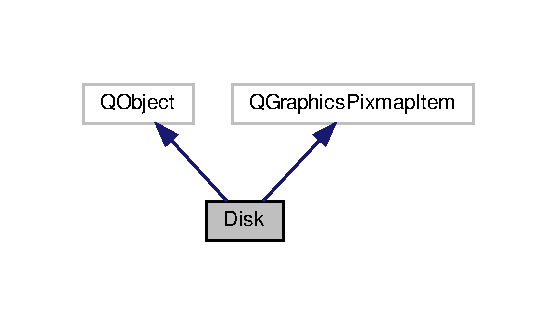
\includegraphics[width=268pt]{classDisk__inherit__graph}
\end{center}
\end{figure}


Collaboration diagram for Disk\+:
\nopagebreak
\begin{figure}[H]
\begin{center}
\leavevmode
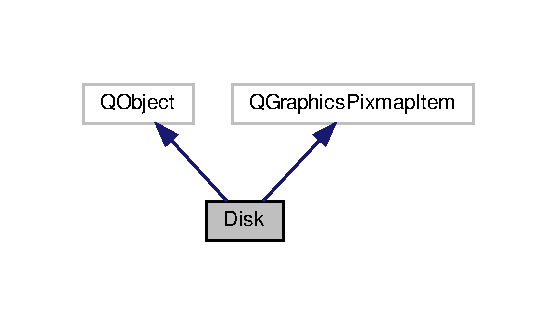
\includegraphics[width=268pt]{classDisk__coll__graph}
\end{center}
\end{figure}
\subsection*{Public Member Functions}
\begin{DoxyCompactItemize}
\item 
\mbox{\Hypertarget{classDisk_a18d1c057a8aa391d3b1df800aae2f87b}\label{classDisk_a18d1c057a8aa391d3b1df800aae2f87b}} 
{\bfseries Disk} (Q\+Object $\ast$parent=nullptr, int game\+Speed=0)
\end{DoxyCompactItemize}
\subsection*{Public Attributes}
\begin{DoxyCompactItemize}
\item 
\mbox{\Hypertarget{classDisk_a711085ff24cfa2046f188a2b8c58a858}\label{classDisk_a711085ff24cfa2046f188a2b8c58a858}} 
int {\bfseries type}
\item 
\mbox{\Hypertarget{classDisk_a8de83d40bc309c5703d7e9a2a10206c3}\label{classDisk_a8de83d40bc309c5703d7e9a2a10206c3}} 
int {\bfseries game\+Speed} =0
\item 
\mbox{\Hypertarget{classDisk_a00d5a6ae66eafcda29d9b9b1baa09604}\label{classDisk_a00d5a6ae66eafcda29d9b9b1baa09604}} 
Q\+Timer $\ast$ {\bfseries timer}
\end{DoxyCompactItemize}


The documentation for this class was generated from the following files\+:\begin{DoxyCompactItemize}
\item 
Game2-\/\+Shooting\+Discs/disk.\+h\item 
Game2-\/\+Shooting\+Discs/disk.\+cpp\end{DoxyCompactItemize}

\hypertarget{classGame1GamePage}{}\section{Game1\+Game\+Page Class Reference}
\label{classGame1GamePage}\index{Game1\+Game\+Page@{Game1\+Game\+Page}}


Inheritance diagram for Game1\+Game\+Page\+:
\nopagebreak
\begin{figure}[H]
\begin{center}
\leavevmode
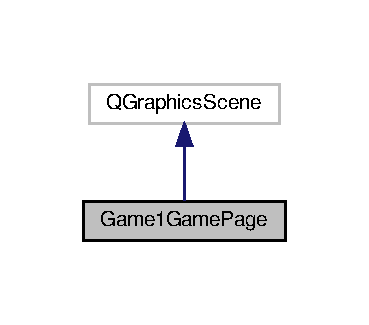
\includegraphics[width=177pt]{classGame1GamePage__inherit__graph}
\end{center}
\end{figure}


Collaboration diagram for Game1\+Game\+Page\+:
\nopagebreak
\begin{figure}[H]
\begin{center}
\leavevmode
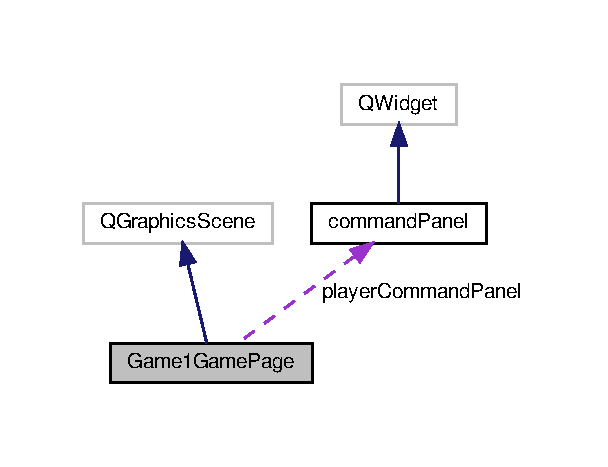
\includegraphics[width=292pt]{classGame1GamePage__coll__graph}
\end{center}
\end{figure}
\subsection*{Public Member Functions}
\begin{DoxyCompactItemize}
\item 
\mbox{\Hypertarget{classGame1GamePage_afaad60ba08c49a7aec3aef5fadb6588c}\label{classGame1GamePage_afaad60ba08c49a7aec3aef5fadb6588c}} 
void \hyperlink{classGame1GamePage_afaad60ba08c49a7aec3aef5fadb6588c}{setup\+Scene} ()
\begin{DoxyCompactList}\small\item\em \hyperlink{classGame1GamePage_afaad60ba08c49a7aec3aef5fadb6588c}{Game1\+Game\+Page\+::setup\+Scene}, sets up the window of game 1 page and its background. \end{DoxyCompactList}\item 
\mbox{\Hypertarget{classGame1GamePage_a7883c5c3eb225ee14e662b8fb73bca69}\label{classGame1GamePage_a7883c5c3eb225ee14e662b8fb73bca69}} 
void \hyperlink{classGame1GamePage_a7883c5c3eb225ee14e662b8fb73bca69}{setup\+Grids} ()
\begin{DoxyCompactList}\small\item\em \hyperlink{classGame1GamePage_a7883c5c3eb225ee14e662b8fb73bca69}{Game1\+Game\+Page\+::setup\+Grids}, sets up the grids of the user and the enemy. \end{DoxyCompactList}\item 
\mbox{\Hypertarget{classGame1GamePage_aa03791d5d0134726886da82236e1fd55}\label{classGame1GamePage_aa03791d5d0134726886da82236e1fd55}} 
void \hyperlink{classGame1GamePage_aa03791d5d0134726886da82236e1fd55}{fill\+Scene} ()
\begin{DoxyCompactList}\small\item\em \hyperlink{classGame1GamePage_aa03791d5d0134726886da82236e1fd55}{Game1\+Game\+Page\+::fill\+Scene}, fills the game scene with all widgets and items. \end{DoxyCompactList}\item 
\mbox{\Hypertarget{classGame1GamePage_ac96dac26541e8e4cffa130d4ceea5117}\label{classGame1GamePage_ac96dac26541e8e4cffa130d4ceea5117}} 
void \hyperlink{classGame1GamePage_ac96dac26541e8e4cffa130d4ceea5117}{setup\+Boats} ()
\begin{DoxyCompactList}\small\item\em \hyperlink{classGame1GamePage_ac96dac26541e8e4cffa130d4ceea5117}{Game1\+Game\+Page\+::setup\+Boats}, sets up boats on the grids of player and enemy. \end{DoxyCompactList}\item 
\mbox{\Hypertarget{classGame1GamePage_a23606106eb189fdbe197c77d717b845c}\label{classGame1GamePage_a23606106eb189fdbe197c77d717b845c}} 
void \hyperlink{classGame1GamePage_a23606106eb189fdbe197c77d717b845c}{setup\+Widgets} ()
\begin{DoxyCompactList}\small\item\em \hyperlink{classGame1GamePage_a23606106eb189fdbe197c77d717b845c}{Game1\+Game\+Page\+::setup\+Widgets}, sets up widgets (Geometry and Appearance) \end{DoxyCompactList}\item 
void \hyperlink{classGame1GamePage_a071eb05d04c53abb1f82fe66ad656040}{setup\+Labels} ()
\begin{DoxyCompactList}\small\item\em \hyperlink{classGame1GamePage_a071eb05d04c53abb1f82fe66ad656040}{Game1\+Game\+Page\+::setup\+Labels}, sets up labels above the main players boats. \end{DoxyCompactList}\item 
void \hyperlink{classGame1GamePage_a55c34bef7d0cb08a617aba01ad556c8c}{setup\+Buttons} ()
\begin{DoxyCompactList}\small\item\em \hyperlink{classGame1GamePage_a55c34bef7d0cb08a617aba01ad556c8c}{Game1\+Game\+Page\+::setup\+Buttons}, set the geometry of buttons that cover the enemy\textquotesingle{}s ships. \end{DoxyCompactList}\item 
Q\+Vector$<$ int $>$ \hyperlink{classGame1GamePage_a47232d81c8e7f96bbf70a16821f86157}{get\+Button\+Position} (Q\+Push\+Button $\ast$button)
\begin{DoxyCompactList}\small\item\em \hyperlink{classGame1GamePage_a47232d81c8e7f96bbf70a16821f86157}{Game1\+Game\+Page\+::get\+Button\+Position}, gets position of the button that the player targets in the enemy\textquotesingle{}s grid(ie. box position in the grid) \end{DoxyCompactList}\item 
bool \hyperlink{classGame1GamePage_aa70f99c3dafab2856e116f1c37efe4e8}{discover\+Block} (int x, int y)
\begin{DoxyCompactList}\small\item\em \hyperlink{classGame1GamePage_aa70f99c3dafab2856e116f1c37efe4e8}{Game1\+Game\+Page\+::discover\+Block}, discovers if under the button lies a part of an enemy ship. \end{DoxyCompactList}\end{DoxyCompactItemize}
\subsection*{Public Attributes}
\begin{DoxyCompactItemize}
\item 
\mbox{\Hypertarget{classGame1GamePage_a85b13ae56a27f03ffc1f60b51243a1cb}\label{classGame1GamePage_a85b13ae56a27f03ffc1f60b51243a1cb}} 
Q\+Graphics\+Pixmap\+Item $\ast$ {\bfseries player1\+Grid}
\item 
\mbox{\Hypertarget{classGame1GamePage_ab2d197eab54acc168da97c35a5603590}\label{classGame1GamePage_ab2d197eab54acc168da97c35a5603590}} 
Q\+Graphics\+Pixmap\+Item $\ast$ {\bfseries player2\+Grid}
\item 
\mbox{\Hypertarget{classGame1GamePage_a749a0f5522a38097547336f9b3afd659}\label{classGame1GamePage_a749a0f5522a38097547336f9b3afd659}} 
Q\+Graphics\+Pixmap\+Item $\ast$ {\bfseries player1\+Boat1}
\item 
\mbox{\Hypertarget{classGame1GamePage_aab142c481a999905443a2099ee13cc85}\label{classGame1GamePage_aab142c481a999905443a2099ee13cc85}} 
Q\+Graphics\+Pixmap\+Item $\ast$ {\bfseries player1\+Boat2}
\item 
\mbox{\Hypertarget{classGame1GamePage_ac04a574400767f267a165a807d445c6b}\label{classGame1GamePage_ac04a574400767f267a165a807d445c6b}} 
Q\+Graphics\+Pixmap\+Item $\ast$ {\bfseries player1\+Boat3}
\item 
\mbox{\Hypertarget{classGame1GamePage_a4d6da6ae1523c45e4b50426f5f26b2de}\label{classGame1GamePage_a4d6da6ae1523c45e4b50426f5f26b2de}} 
Q\+Graphics\+Pixmap\+Item $\ast$ {\bfseries player2\+Boat1}
\item 
\mbox{\Hypertarget{classGame1GamePage_aa8ae0f2b64f18151ad26d897d2c9601e}\label{classGame1GamePage_aa8ae0f2b64f18151ad26d897d2c9601e}} 
Q\+Graphics\+Pixmap\+Item $\ast$ {\bfseries player2\+Boat2}
\item 
\mbox{\Hypertarget{classGame1GamePage_ab21a2665749eabb61121742550caa038}\label{classGame1GamePage_ab21a2665749eabb61121742550caa038}} 
Q\+Graphics\+Pixmap\+Item $\ast$ {\bfseries player2\+Boat3}
\item 
\mbox{\Hypertarget{classGame1GamePage_ae54a83518f95a02ab218198a6b45a6d2}\label{classGame1GamePage_ae54a83518f95a02ab218198a6b45a6d2}} 
Q\+Graphics\+Pixmap\+Item $\ast$ {\bfseries player2\+Boat4}
\item 
\mbox{\Hypertarget{classGame1GamePage_a3518354f4ea9e7f8ee3b59b0cee3faed}\label{classGame1GamePage_a3518354f4ea9e7f8ee3b59b0cee3faed}} 
Q\+Graphics\+Pixmap\+Item $\ast$ {\bfseries player2\+Boat5}
\item 
\mbox{\Hypertarget{classGame1GamePage_a54fc09dfc5e07a30650a70b56ea03b13}\label{classGame1GamePage_a54fc09dfc5e07a30650a70b56ea03b13}} 
Q\+Graphics\+Pixmap\+Item $\ast$ {\bfseries player2\+Boat6}
\item 
\mbox{\Hypertarget{classGame1GamePage_a7d49025fb26d96a30bf57dd3d0df4591}\label{classGame1GamePage_a7d49025fb26d96a30bf57dd3d0df4591}} 
\hyperlink{classcommandPanel}{command\+Panel} $\ast$ {\bfseries player\+Command\+Panel}
\item 
\mbox{\Hypertarget{classGame1GamePage_ae8b91ab81442125ecb68f53c75ad33d7}\label{classGame1GamePage_ae8b91ab81442125ecb68f53c75ad33d7}} 
Q\+Label $\ast$ {\bfseries G\+C\+P\+Label}
\item 
\mbox{\Hypertarget{classGame1GamePage_af2a336703f379f45151221a66b5cbe21}\label{classGame1GamePage_af2a336703f379f45151221a66b5cbe21}} 
Q\+Label $\ast$ {\bfseries B\+C\+P\+Label}
\item 
\mbox{\Hypertarget{classGame1GamePage_aba0851ff24c3db694ae5200c3739a465}\label{classGame1GamePage_aba0851ff24c3db694ae5200c3739a465}} 
Q\+Label $\ast$ {\bfseries correct\+Answer\+No}
\item 
\mbox{\Hypertarget{classGame1GamePage_ab55f7f14e0d8c73a24b7edafd59b90d7}\label{classGame1GamePage_ab55f7f14e0d8c73a24b7edafd59b90d7}} 
Q\+Label $\ast$ {\bfseries incorrect\+Answer\+No}
\item 
\mbox{\Hypertarget{classGame1GamePage_af412a77fccdebe1d0a4f07699174f08c}\label{classGame1GamePage_af412a77fccdebe1d0a4f07699174f08c}} 
Q\+Label $\ast$ {\bfseries game\+Status}
\item 
\mbox{\Hypertarget{classGame1GamePage_acfa716f34e6b3fa19392a69e9022af35}\label{classGame1GamePage_acfa716f34e6b3fa19392a69e9022af35}} 
Q\+Push\+Button $\ast$ {\bfseries button00}
\item 
\mbox{\Hypertarget{classGame1GamePage_a11bcc55eacd28fe6117994114e8c8134}\label{classGame1GamePage_a11bcc55eacd28fe6117994114e8c8134}} 
Q\+Push\+Button $\ast$ {\bfseries button01}
\item 
\mbox{\Hypertarget{classGame1GamePage_a4d1752207e24d7413bc516202c48e2c4}\label{classGame1GamePage_a4d1752207e24d7413bc516202c48e2c4}} 
Q\+Push\+Button $\ast$ {\bfseries button02}
\item 
\mbox{\Hypertarget{classGame1GamePage_ae40d26d7fb7cebf2984588d87ec63841}\label{classGame1GamePage_ae40d26d7fb7cebf2984588d87ec63841}} 
Q\+Push\+Button $\ast$ {\bfseries button03}
\item 
\mbox{\Hypertarget{classGame1GamePage_a58e1b7725a4afacaf0e054827cb0a36c}\label{classGame1GamePage_a58e1b7725a4afacaf0e054827cb0a36c}} 
Q\+Push\+Button $\ast$ {\bfseries button10}
\item 
\mbox{\Hypertarget{classGame1GamePage_a61f6ebba2ceb6a57c8d044bfc65db125}\label{classGame1GamePage_a61f6ebba2ceb6a57c8d044bfc65db125}} 
Q\+Push\+Button $\ast$ {\bfseries button11}
\item 
\mbox{\Hypertarget{classGame1GamePage_a47d69a0222596117d101eb5c33acc1fd}\label{classGame1GamePage_a47d69a0222596117d101eb5c33acc1fd}} 
Q\+Push\+Button $\ast$ {\bfseries button12}
\item 
\mbox{\Hypertarget{classGame1GamePage_a0166c20f94a4d1a3e41e566ed1e68379}\label{classGame1GamePage_a0166c20f94a4d1a3e41e566ed1e68379}} 
Q\+Push\+Button $\ast$ {\bfseries button13}
\item 
\mbox{\Hypertarget{classGame1GamePage_a844db9ee5ad34b0ad90363781224b7f6}\label{classGame1GamePage_a844db9ee5ad34b0ad90363781224b7f6}} 
Q\+Push\+Button $\ast$ {\bfseries button20}
\item 
\mbox{\Hypertarget{classGame1GamePage_a98f90a0aed02ba916679ed4cfeb56666}\label{classGame1GamePage_a98f90a0aed02ba916679ed4cfeb56666}} 
Q\+Push\+Button $\ast$ {\bfseries button21}
\item 
\mbox{\Hypertarget{classGame1GamePage_a009b058320a7f09445a238ec843b56f0}\label{classGame1GamePage_a009b058320a7f09445a238ec843b56f0}} 
Q\+Push\+Button $\ast$ {\bfseries button22}
\item 
\mbox{\Hypertarget{classGame1GamePage_afba915558c68516883c70ce0162948fd}\label{classGame1GamePage_afba915558c68516883c70ce0162948fd}} 
Q\+Push\+Button $\ast$ {\bfseries button23}
\item 
\mbox{\Hypertarget{classGame1GamePage_a7e3cae8c9a7af349f909d2d793c07241}\label{classGame1GamePage_a7e3cae8c9a7af349f909d2d793c07241}} 
Q\+Push\+Button $\ast$ {\bfseries button30}
\item 
\mbox{\Hypertarget{classGame1GamePage_a2d98ecb78b9d0750a9de9d220404e644}\label{classGame1GamePage_a2d98ecb78b9d0750a9de9d220404e644}} 
Q\+Push\+Button $\ast$ {\bfseries button31}
\item 
\mbox{\Hypertarget{classGame1GamePage_a611314e83752c0045ddaeb4bf975c69d}\label{classGame1GamePage_a611314e83752c0045ddaeb4bf975c69d}} 
Q\+Push\+Button $\ast$ {\bfseries button32}
\item 
\mbox{\Hypertarget{classGame1GamePage_acdae6626152d3a4862a6d29f1442c658}\label{classGame1GamePage_acdae6626152d3a4862a6d29f1442c658}} 
Q\+Push\+Button $\ast$ {\bfseries button33}
\item 
\mbox{\Hypertarget{classGame1GamePage_a2b2c1855a0da027deec667c11fb7ec4e}\label{classGame1GamePage_a2b2c1855a0da027deec667c11fb7ec4e}} 
Q\+Label $\ast$ {\bfseries boat1\+Part1\+Label}
\item 
\mbox{\Hypertarget{classGame1GamePage_abee94a06eb70b1d56f275a827a3ea8c1}\label{classGame1GamePage_abee94a06eb70b1d56f275a827a3ea8c1}} 
Q\+Label $\ast$ {\bfseries boat1\+Part2\+Label}
\item 
\mbox{\Hypertarget{classGame1GamePage_ab7a34c4aeb0dcee242f7552bfe365c0e}\label{classGame1GamePage_ab7a34c4aeb0dcee242f7552bfe365c0e}} 
Q\+Label $\ast$ {\bfseries boat1\+Part3\+Label}
\item 
\mbox{\Hypertarget{classGame1GamePage_add9cc20ff675a3af2214434ade38e812}\label{classGame1GamePage_add9cc20ff675a3af2214434ade38e812}} 
Q\+Label $\ast$ {\bfseries boat2\+Label}
\item 
\mbox{\Hypertarget{classGame1GamePage_a24c75dff3dfec462f172896e2044d971}\label{classGame1GamePage_a24c75dff3dfec462f172896e2044d971}} 
Q\+Label $\ast$ {\bfseries boat3\+Label}
\item 
\mbox{\Hypertarget{classGame1GamePage_a62f04a32d802bbe089451d469fe77f25}\label{classGame1GamePage_a62f04a32d802bbe089451d469fe77f25}} 
int {\bfseries bad\+Answers}
\item 
\mbox{\Hypertarget{classGame1GamePage_ad70ff23f6015867d84e69e432aaffac7}\label{classGame1GamePage_ad70ff23f6015867d84e69e432aaffac7}} 
Q\+Vector$<$ Q\+Vector$<$ Q\+Push\+Button $\ast$ $>$ $>$ {\bfseries grid\+Buttons}
\item 
\mbox{\Hypertarget{classGame1GamePage_a61d460be2f955377e656d7bfbf58aec1}\label{classGame1GamePage_a61d460be2f955377e656d7bfbf58aec1}} 
Q\+Vector$<$ Q\+Vector$<$ bool $>$ $>$ {\bfseries user\+Boat\+Positions}
\item 
\mbox{\Hypertarget{classGame1GamePage_a4fb0a4e7d44b86217db2775ae38b0c88}\label{classGame1GamePage_a4fb0a4e7d44b86217db2775ae38b0c88}} 
Q\+Vector$<$ Q\+Vector$<$ bool $>$ $>$ {\bfseries enemy\+Boat\+Positions}
\item 
\mbox{\Hypertarget{classGame1GamePage_a59e7ce71a4b0672fb49e6cdf927baac4}\label{classGame1GamePage_a59e7ce71a4b0672fb49e6cdf927baac4}} 
Q\+String {\bfseries last\+Box\+Chosen}
\item 
\mbox{\Hypertarget{classGame1GamePage_ac2a5bcec1e786a3ce95dff0ce2c0a8a3}\label{classGame1GamePage_ac2a5bcec1e786a3ce95dff0ce2c0a8a3}} 
Q\+Push\+Button $\ast$ {\bfseries home}
\item 
\mbox{\Hypertarget{classGame1GamePage_afa6f1549edcf760257511c2e14862e6b}\label{classGame1GamePage_afa6f1549edcf760257511c2e14862e6b}} 
bool {\bfseries end\+Game} = false
\end{DoxyCompactItemize}


\subsection{Member Function Documentation}
\mbox{\Hypertarget{classGame1GamePage_aa70f99c3dafab2856e116f1c37efe4e8}\label{classGame1GamePage_aa70f99c3dafab2856e116f1c37efe4e8}} 
\index{Game1\+Game\+Page@{Game1\+Game\+Page}!discover\+Block@{discover\+Block}}
\index{discover\+Block@{discover\+Block}!Game1\+Game\+Page@{Game1\+Game\+Page}}
\subsubsection{\texorpdfstring{discover\+Block()}{discoverBlock()}}
{\footnotesize\ttfamily bool Game1\+Game\+Page\+::discover\+Block (\begin{DoxyParamCaption}\item[{int}]{x,  }\item[{int}]{y }\end{DoxyParamCaption})}



\hyperlink{classGame1GamePage_aa70f99c3dafab2856e116f1c37efe4e8}{Game1\+Game\+Page\+::discover\+Block}, discovers if under the button lies a part of an enemy ship. 


\begin{DoxyParams}{Parameters}
{\em x} & representing the x position. \\
\hline
{\em y} & representing the y position. \\
\hline
\end{DoxyParams}
\begin{DoxyReturn}{Returns}
true if ship found, false otherwise. 
\end{DoxyReturn}
\mbox{\Hypertarget{classGame1GamePage_a47232d81c8e7f96bbf70a16821f86157}\label{classGame1GamePage_a47232d81c8e7f96bbf70a16821f86157}} 
\index{Game1\+Game\+Page@{Game1\+Game\+Page}!get\+Button\+Position@{get\+Button\+Position}}
\index{get\+Button\+Position@{get\+Button\+Position}!Game1\+Game\+Page@{Game1\+Game\+Page}}
\subsubsection{\texorpdfstring{get\+Button\+Position()}{getButtonPosition()}}
{\footnotesize\ttfamily Q\+Vector$<$ int $>$ Game1\+Game\+Page\+::get\+Button\+Position (\begin{DoxyParamCaption}\item[{Q\+Push\+Button $\ast$}]{button }\end{DoxyParamCaption})}



\hyperlink{classGame1GamePage_a47232d81c8e7f96bbf70a16821f86157}{Game1\+Game\+Page\+::get\+Button\+Position}, gets position of the button that the player targets in the enemy\textquotesingle{}s grid(ie. box position in the grid) 


\begin{DoxyParams}{Parameters}
{\em button} & \\
\hline
\end{DoxyParams}
\begin{DoxyReturn}{Returns}
Qvector contianing the x,y coordinates of the button targeted. In case button not in grid return vector containing -\/1. 
\end{DoxyReturn}
\mbox{\Hypertarget{classGame1GamePage_a55c34bef7d0cb08a617aba01ad556c8c}\label{classGame1GamePage_a55c34bef7d0cb08a617aba01ad556c8c}} 
\index{Game1\+Game\+Page@{Game1\+Game\+Page}!setup\+Buttons@{setup\+Buttons}}
\index{setup\+Buttons@{setup\+Buttons}!Game1\+Game\+Page@{Game1\+Game\+Page}}
\subsubsection{\texorpdfstring{setup\+Buttons()}{setupButtons()}}
{\footnotesize\ttfamily void Game1\+Game\+Page\+::setup\+Buttons (\begin{DoxyParamCaption}{ }\end{DoxyParamCaption})}



\hyperlink{classGame1GamePage_a55c34bef7d0cb08a617aba01ad556c8c}{Game1\+Game\+Page\+::setup\+Buttons}, set the geometry of buttons that cover the enemy\textquotesingle{}s ships. 

The buttons are not clickable, the are just present to cover the enemy ships.\mbox{\Hypertarget{classGame1GamePage_a071eb05d04c53abb1f82fe66ad656040}\label{classGame1GamePage_a071eb05d04c53abb1f82fe66ad656040}} 
\index{Game1\+Game\+Page@{Game1\+Game\+Page}!setup\+Labels@{setup\+Labels}}
\index{setup\+Labels@{setup\+Labels}!Game1\+Game\+Page@{Game1\+Game\+Page}}
\subsubsection{\texorpdfstring{setup\+Labels()}{setupLabels()}}
{\footnotesize\ttfamily void Game1\+Game\+Page\+::setup\+Labels (\begin{DoxyParamCaption}{ }\end{DoxyParamCaption})}



\hyperlink{classGame1GamePage_a071eb05d04c53abb1f82fe66ad656040}{Game1\+Game\+Page\+::setup\+Labels}, sets up labels above the main players boats. 

These labels get recoloured to red once the enemy hits one of the main player\textquotesingle{}s boats. 

The documentation for this class was generated from the following files\+:\begin{DoxyCompactItemize}
\item 
Game1-\/\+Battle\+Ship/game1gamepage.\+h\item 
Game1-\/\+Battle\+Ship/game1gamepage.\+cpp\end{DoxyCompactItemize}

\hypertarget{classGame1View}{}\section{Game1\+View Class Reference}
\label{classGame1View}\index{Game1\+View@{Game1\+View}}


Inheritance diagram for Game1\+View\+:
\nopagebreak
\begin{figure}[H]
\begin{center}
\leavevmode
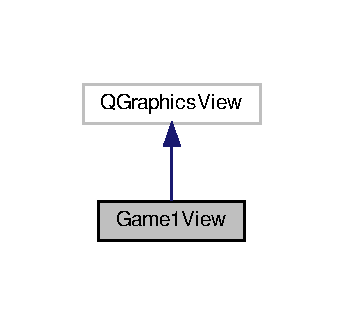
\includegraphics[width=165pt]{classGame1View__inherit__graph}
\end{center}
\end{figure}


Collaboration diagram for Game1\+View\+:
\nopagebreak
\begin{figure}[H]
\begin{center}
\leavevmode
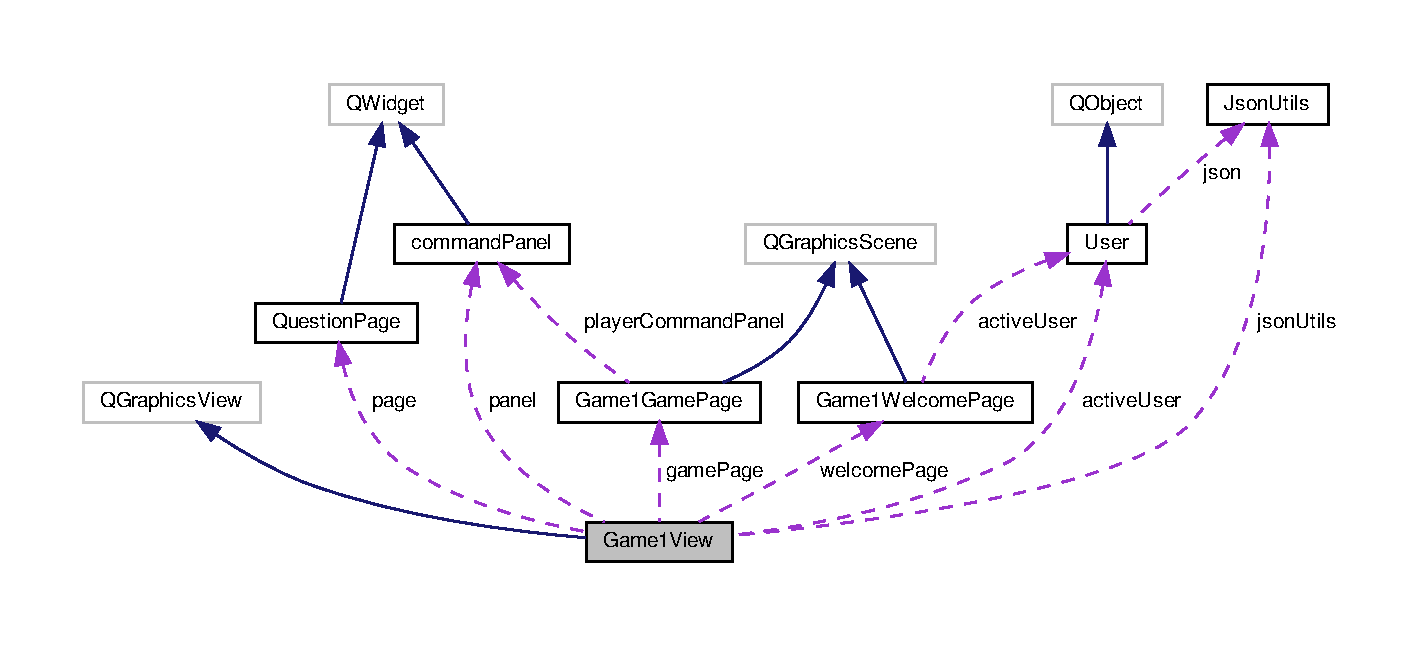
\includegraphics[width=350pt]{classGame1View__coll__graph}
\end{center}
\end{figure}
\subsection*{Public Slots}
\begin{DoxyCompactItemize}
\item 
\mbox{\Hypertarget{classGame1View_a8a96444a8609be01e432f594ef9d5278}\label{classGame1View_a8a96444a8609be01e432f594ef9d5278}} 
void \hyperlink{classGame1View_a8a96444a8609be01e432f594ef9d5278}{start\+Game} ()
\begin{DoxyCompactList}\small\item\em \hyperlink{classGame1View_a8a96444a8609be01e432f594ef9d5278}{Game1\+View\+::start\+Game}, starts the game and changes scene to game\+Page. \end{DoxyCompactList}\item 
\mbox{\Hypertarget{classGame1View_a400e6a38b7059f5482af91c7526ecd81}\label{classGame1View_a400e6a38b7059f5482af91c7526ecd81}} 
void \hyperlink{classGame1View_a400e6a38b7059f5482af91c7526ecd81}{correct\+Answer} ()
\begin{DoxyCompactList}\small\item\em \hyperlink{classGame1View_a400e6a38b7059f5482af91c7526ecd81}{Game1\+View\+::correct\+Answer}, handles case of user entering a correct answer. \end{DoxyCompactList}\item 
\mbox{\Hypertarget{classGame1View_a3339f02c7248a8524ec46f1b3b51406c}\label{classGame1View_a3339f02c7248a8524ec46f1b3b51406c}} 
void \hyperlink{classGame1View_a3339f02c7248a8524ec46f1b3b51406c}{wrong\+Answer} ()
\begin{DoxyCompactList}\small\item\em \hyperlink{classGame1View_a3339f02c7248a8524ec46f1b3b51406c}{Game1\+View\+::wrong\+Answer}, handles case of user entering a wrong answer. \end{DoxyCompactList}\item 
\mbox{\Hypertarget{classGame1View_ad9ad0551c9087ebe58db95e049b27300}\label{classGame1View_ad9ad0551c9087ebe58db95e049b27300}} 
void \hyperlink{classGame1View_ad9ad0551c9087ebe58db95e049b27300}{hit\+Home} ()
\begin{DoxyCompactList}\small\item\em \hyperlink{classGame1View_ad9ad0551c9087ebe58db95e049b27300}{Game1\+View\+::hit\+Home}, handles case when user receives a hit from enemy. \end{DoxyCompactList}\item 
\mbox{\Hypertarget{classGame1View_ac6867d86cfd279dd2a4723274af33564}\label{classGame1View_ac6867d86cfd279dd2a4723274af33564}} 
void \hyperlink{classGame1View_ac6867d86cfd279dd2a4723274af33564}{attack} ()
\begin{DoxyCompactList}\small\item\em \hyperlink{classGame1View_ac6867d86cfd279dd2a4723274af33564}{Game1\+View\+::attack}, takes input from command panel and attacks respective box in grid. \end{DoxyCompactList}\item 
\mbox{\Hypertarget{classGame1View_a6836a99c180e8dab53af1c8575993dec}\label{classGame1View_a6836a99c180e8dab53af1c8575993dec}} 
void \hyperlink{classGame1View_a6836a99c180e8dab53af1c8575993dec}{go\+To\+Home} ()
\begin{DoxyCompactList}\small\item\em \hyperlink{classGame1View_a6836a99c180e8dab53af1c8575993dec}{Game1\+View\+::go\+To\+Home}, returns the user to home page to choose between the 2 games. \end{DoxyCompactList}\end{DoxyCompactItemize}
\subsection*{Public Member Functions}
\begin{DoxyCompactItemize}
\item 
void \hyperlink{classGame1View_a013dc48c98ecb2c52516d433aac4a112}{key\+Press\+Event} (Q\+Key\+Event $\ast$event)
\begin{DoxyCompactList}\small\item\em \hyperlink{classGame1View_a013dc48c98ecb2c52516d433aac4a112}{Game1\+View\+::key\+Press\+Event}, starts the game when F1 Button is pressed. \end{DoxyCompactList}\item 
\mbox{\Hypertarget{classGame1View_a2209a714e878e9654d980006360bc855}\label{classGame1View_a2209a714e878e9654d980006360bc855}} 
void \hyperlink{classGame1View_a2209a714e878e9654d980006360bc855}{connect\+Buttons} ()
\begin{DoxyCompactList}\small\item\em \hyperlink{classGame1View_a2209a714e878e9654d980006360bc855}{Game1\+View\+::connect\+Buttons}, connects multiple buttons to their corresponding slots. \end{DoxyCompactList}\item 
\mbox{\Hypertarget{classGame1View_abb63a59f922e1104fa88f3c7561831b5}\label{classGame1View_abb63a59f922e1104fa88f3c7561831b5}} 
void \hyperlink{classGame1View_abb63a59f922e1104fa88f3c7561831b5}{clear\+Question\+Page} ()
\begin{DoxyCompactList}\small\item\em \hyperlink{classGame1View_abb63a59f922e1104fa88f3c7561831b5}{Game1\+View\+::clear\+Question\+Page}, clears question page when the game ends. \end{DoxyCompactList}\item 
\mbox{\Hypertarget{classGame1View_a0d292597798333a5465a540f38d6fe86}\label{classGame1View_a0d292597798333a5465a540f38d6fe86}} 
void \hyperlink{classGame1View_a0d292597798333a5465a540f38d6fe86}{check\+Curr\+Game\+Scores} ()
\begin{DoxyCompactList}\small\item\em \hyperlink{classGame1View_a0d292597798333a5465a540f38d6fe86}{Game1\+View\+::check\+Curr\+Game\+Scores}, checks the in-\/game scores of the active game. \end{DoxyCompactList}\item 
void \hyperlink{classGame1View_ad1c25c3de31c9b0181af7e837284b0d5}{end\+Current\+Game} (bool win\+Or\+Lose)
\begin{DoxyCompactList}\small\item\em \hyperlink{classGame1View_ad1c25c3de31c9b0181af7e837284b0d5}{Game1\+View\+::end\+Current\+Game}, ends game when user either wins or loses. \end{DoxyCompactList}\item 
void \hyperlink{classGame1View_aa5ed1a0bd0034b87c20c649c3950a337}{reveal\+Box} (int x, int y)
\begin{DoxyCompactList}\small\item\em \hyperlink{classGame1View_aa5ed1a0bd0034b87c20c649c3950a337}{Game1\+View\+::reveal\+Box}, reveals box if the user answered its corresponding question correctly, or if no ship is found under the box. \end{DoxyCompactList}\item 
void \hyperlink{classGame1View_a0739a9638e33409f70bc1ab4337e3c83}{strike\+Box} (int x, int y)
\begin{DoxyCompactList}\small\item\em \hyperlink{classGame1View_a0739a9638e33409f70bc1ab4337e3c83}{Game1\+View\+::strike\+Box}, marks box as red if user misses the correct answer to the question. \end{DoxyCompactList}\end{DoxyCompactItemize}
\subsection*{Public Attributes}
\begin{DoxyCompactItemize}
\item 
\mbox{\Hypertarget{classGame1View_ac82e9873bf8f94387d5fbc1a3320554c}\label{classGame1View_ac82e9873bf8f94387d5fbc1a3320554c}} 
\hyperlink{classUser}{User} $\ast$ {\bfseries active\+User} = N\+U\+LL
\item 
\mbox{\Hypertarget{classGame1View_aaa32a67d71d09ead7aa657b5197b7074}\label{classGame1View_aaa32a67d71d09ead7aa657b5197b7074}} 
\hyperlink{classGame1WelcomePage}{Game1\+Welcome\+Page} $\ast$ {\bfseries welcome\+Page}
\item 
\mbox{\Hypertarget{classGame1View_a674af281b3cd32678f0196b6ecdc6da3}\label{classGame1View_a674af281b3cd32678f0196b6ecdc6da3}} 
\hyperlink{classGame1GamePage}{Game1\+Game\+Page} $\ast$ {\bfseries game\+Page}
\item 
\mbox{\Hypertarget{classGame1View_a15bd450042b3dbe0b4506df138167395}\label{classGame1View_a15bd450042b3dbe0b4506df138167395}} 
\hyperlink{classQuestionPage}{Question\+Page} $\ast$ {\bfseries page}
\item 
\mbox{\Hypertarget{classGame1View_ab4c444271424b0468ea2538c94c6c720}\label{classGame1View_ab4c444271424b0468ea2538c94c6c720}} 
Q\+Vector$<$ bool $>$ {\bfseries current\+Game\+Scores}
\item 
\mbox{\Hypertarget{classGame1View_a7d67e8caaac9295fa0c07b9da043a317}\label{classGame1View_a7d67e8caaac9295fa0c07b9da043a317}} 
\hyperlink{classJsonUtils}{Json\+Utils} $\ast$ {\bfseries json\+Utils}
\item 
\mbox{\Hypertarget{classGame1View_a11c488d83ea7edf0c9b0ff9c08c0573a}\label{classGame1View_a11c488d83ea7edf0c9b0ff9c08c0573a}} 
\hyperlink{classcommandPanel}{command\+Panel} $\ast$ {\bfseries panel}
\item 
\mbox{\Hypertarget{classGame1View_a0d70035d5b718d7c5a3a016a23e5f38e}\label{classGame1View_a0d70035d5b718d7c5a3a016a23e5f38e}} 
Q\+Graphics\+View $\ast$ {\bfseries app\+Main\+View}
\end{DoxyCompactItemize}


\subsection{Member Function Documentation}
\mbox{\Hypertarget{classGame1View_ad1c25c3de31c9b0181af7e837284b0d5}\label{classGame1View_ad1c25c3de31c9b0181af7e837284b0d5}} 
\index{Game1\+View@{Game1\+View}!end\+Current\+Game@{end\+Current\+Game}}
\index{end\+Current\+Game@{end\+Current\+Game}!Game1\+View@{Game1\+View}}
\subsubsection{\texorpdfstring{end\+Current\+Game()}{endCurrentGame()}}
{\footnotesize\ttfamily void Game1\+View\+::end\+Current\+Game (\begin{DoxyParamCaption}\item[{bool}]{win\+Or\+Lose }\end{DoxyParamCaption})}



\hyperlink{classGame1View_ad1c25c3de31c9b0181af7e837284b0d5}{Game1\+View\+::end\+Current\+Game}, ends game when user either wins or loses. 


\begin{DoxyParams}{Parameters}
{\em win\+Or\+Lose,true} & for winning and false for losing \\
\hline
\end{DoxyParams}
\mbox{\Hypertarget{classGame1View_a013dc48c98ecb2c52516d433aac4a112}\label{classGame1View_a013dc48c98ecb2c52516d433aac4a112}} 
\index{Game1\+View@{Game1\+View}!key\+Press\+Event@{key\+Press\+Event}}
\index{key\+Press\+Event@{key\+Press\+Event}!Game1\+View@{Game1\+View}}
\subsubsection{\texorpdfstring{key\+Press\+Event()}{keyPressEvent()}}
{\footnotesize\ttfamily void Game1\+View\+::key\+Press\+Event (\begin{DoxyParamCaption}\item[{Q\+Key\+Event $\ast$}]{event }\end{DoxyParamCaption})}



\hyperlink{classGame1View_a013dc48c98ecb2c52516d433aac4a112}{Game1\+View\+::key\+Press\+Event}, starts the game when F1 Button is pressed. 


\begin{DoxyParams}{Parameters}
{\em event} & \\
\hline
\end{DoxyParams}
\mbox{\Hypertarget{classGame1View_aa5ed1a0bd0034b87c20c649c3950a337}\label{classGame1View_aa5ed1a0bd0034b87c20c649c3950a337}} 
\index{Game1\+View@{Game1\+View}!reveal\+Box@{reveal\+Box}}
\index{reveal\+Box@{reveal\+Box}!Game1\+View@{Game1\+View}}
\subsubsection{\texorpdfstring{reveal\+Box()}{revealBox()}}
{\footnotesize\ttfamily void Game1\+View\+::reveal\+Box (\begin{DoxyParamCaption}\item[{int}]{x,  }\item[{int}]{y }\end{DoxyParamCaption})}



\hyperlink{classGame1View_aa5ed1a0bd0034b87c20c649c3950a337}{Game1\+View\+::reveal\+Box}, reveals box if the user answered its corresponding question correctly, or if no ship is found under the box. 


\begin{DoxyParams}{Parameters}
{\em x} & representing the x position of the box \\
\hline
{\em y} & representing the y position of the box \\
\hline
\end{DoxyParams}
\mbox{\Hypertarget{classGame1View_a0739a9638e33409f70bc1ab4337e3c83}\label{classGame1View_a0739a9638e33409f70bc1ab4337e3c83}} 
\index{Game1\+View@{Game1\+View}!strike\+Box@{strike\+Box}}
\index{strike\+Box@{strike\+Box}!Game1\+View@{Game1\+View}}
\subsubsection{\texorpdfstring{strike\+Box()}{strikeBox()}}
{\footnotesize\ttfamily void Game1\+View\+::strike\+Box (\begin{DoxyParamCaption}\item[{int}]{x,  }\item[{int}]{y }\end{DoxyParamCaption})}



\hyperlink{classGame1View_a0739a9638e33409f70bc1ab4337e3c83}{Game1\+View\+::strike\+Box}, marks box as red if user misses the correct answer to the question. 


\begin{DoxyParams}{Parameters}
{\em x} & representing the x coordinate of the box \\
\hline
{\em y} & representing the y coordinate of the box \\
\hline
\end{DoxyParams}


The documentation for this class was generated from the following files\+:\begin{DoxyCompactItemize}
\item 
Game1-\/\+Battle\+Ship/game1view.\+h\item 
Game1-\/\+Battle\+Ship/game1view.\+cpp\end{DoxyCompactItemize}

\hypertarget{classGame1WelcomePage}{}\section{Game1\+Welcome\+Page Class Reference}
\label{classGame1WelcomePage}\index{Game1\+Welcome\+Page@{Game1\+Welcome\+Page}}


Inheritance diagram for Game1\+Welcome\+Page\+:
\nopagebreak
\begin{figure}[H]
\begin{center}
\leavevmode
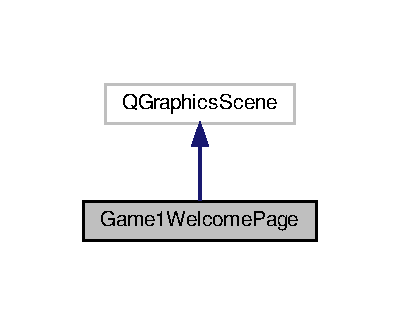
\includegraphics[width=192pt]{classGame1WelcomePage__inherit__graph}
\end{center}
\end{figure}


Collaboration diagram for Game1\+Welcome\+Page\+:
\nopagebreak
\begin{figure}[H]
\begin{center}
\leavevmode
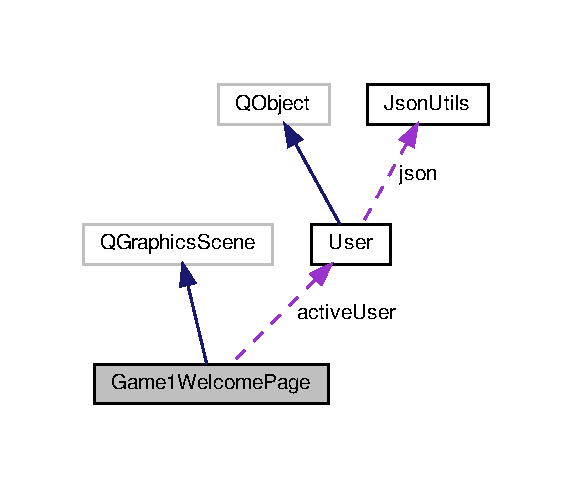
\includegraphics[width=275pt]{classGame1WelcomePage__coll__graph}
\end{center}
\end{figure}
\subsection*{Public Member Functions}
\begin{DoxyCompactItemize}
\item 
\mbox{\Hypertarget{classGame1WelcomePage_adb52f15e9d1da8800d544924d8166bf2}\label{classGame1WelcomePage_adb52f15e9d1da8800d544924d8166bf2}} 
void \hyperlink{classGame1WelcomePage_adb52f15e9d1da8800d544924d8166bf2}{setup\+Scene} ()
\begin{DoxyCompactList}\small\item\em \hyperlink{classGame1WelcomePage_adb52f15e9d1da8800d544924d8166bf2}{Game1\+Welcome\+Page\+::setup\+Scene}, sets up the scene for the welcome page of game 1. \end{DoxyCompactList}\end{DoxyCompactItemize}
\subsection*{Public Attributes}
\begin{DoxyCompactItemize}
\item 
\mbox{\Hypertarget{classGame1WelcomePage_af22e39d821428cef70ea1f7f14bbf07e}\label{classGame1WelcomePage_af22e39d821428cef70ea1f7f14bbf07e}} 
\hyperlink{classUser}{User} $\ast$ {\bfseries active\+User} = N\+U\+LL
\item 
\mbox{\Hypertarget{classGame1WelcomePage_ad5a2341f2f1f8cbcd1e177c8324f8ef0}\label{classGame1WelcomePage_ad5a2341f2f1f8cbcd1e177c8324f8ef0}} 
Q\+Label $\ast$ {\bfseries game\+Name}
\item 
\mbox{\Hypertarget{classGame1WelcomePage_adf4925039198d5fa91928de80553b1fd}\label{classGame1WelcomePage_adf4925039198d5fa91928de80553b1fd}} 
Q\+Label $\ast$ {\bfseries game\+Insructions}
\item 
\mbox{\Hypertarget{classGame1WelcomePage_a3ccd25fb9e2ca9ca91a18c0bbb31a860}\label{classGame1WelcomePage_a3ccd25fb9e2ca9ca91a18c0bbb31a860}} 
Q\+Push\+Button $\ast$ {\bfseries play\+Game}
\end{DoxyCompactItemize}


The documentation for this class was generated from the following files\+:\begin{DoxyCompactItemize}
\item 
Game1-\/\+Battle\+Ship/game1welcomepage.\+h\item 
Game1-\/\+Battle\+Ship/game1welcomepage.\+cpp\end{DoxyCompactItemize}

\hypertarget{classGame2GamePage}{}\section{Game2\+Game\+Page Class Reference}
\label{classGame2GamePage}\index{Game2\+Game\+Page@{Game2\+Game\+Page}}


Inheritance diagram for Game2\+Game\+Page\+:
\nopagebreak
\begin{figure}[H]
\begin{center}
\leavevmode
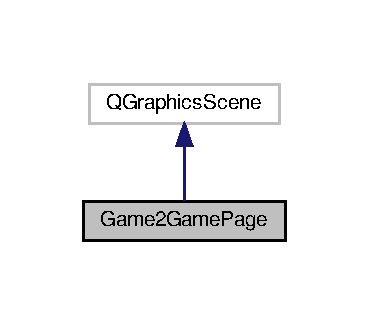
\includegraphics[width=177pt]{classGame2GamePage__inherit__graph}
\end{center}
\end{figure}


Collaboration diagram for Game2\+Game\+Page\+:
\nopagebreak
\begin{figure}[H]
\begin{center}
\leavevmode
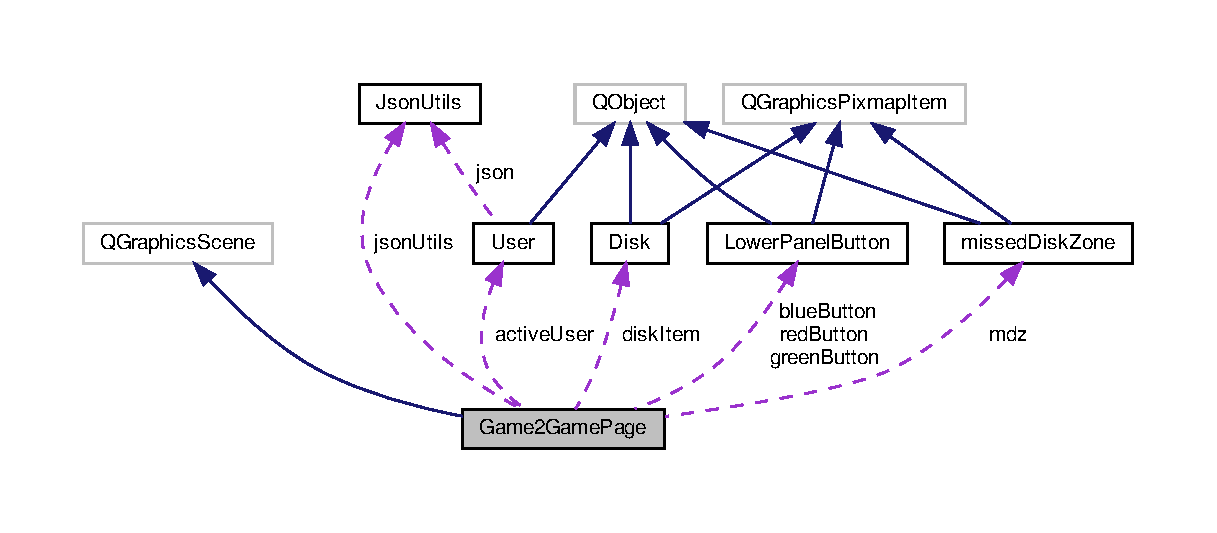
\includegraphics[width=350pt]{classGame2GamePage__coll__graph}
\end{center}
\end{figure}
\subsection*{Public Slots}
\begin{DoxyCompactItemize}
\item 
\mbox{\Hypertarget{classGame2GamePage_a17a93aeabdf272879dd814b0381bfca8}\label{classGame2GamePage_a17a93aeabdf272879dd814b0381bfca8}} 
void \hyperlink{classGame2GamePage_a17a93aeabdf272879dd814b0381bfca8}{add\+Disk} ()
\begin{DoxyCompactList}\small\item\em \hyperlink{classGame2GamePage_a17a93aeabdf272879dd814b0381bfca8}{Game2\+Game\+Page\+::add\+Disk}, creates and adds a disk on the game boards. \end{DoxyCompactList}\item 
\mbox{\Hypertarget{classGame2GamePage_a7f2480ad602fe9e6f4e13f7bd86a8fe5}\label{classGame2GamePage_a7f2480ad602fe9e6f4e13f7bd86a8fe5}} 
void \hyperlink{classGame2GamePage_a7f2480ad602fe9e6f4e13f7bd86a8fe5}{check\+Missed\+Disks} ()
\begin{DoxyCompactList}\small\item\em \hyperlink{classGame2GamePage_a7f2480ad602fe9e6f4e13f7bd86a8fe5}{Game2\+Game\+Page\+::check\+Missed\+Disks}, function that checks if a disk made it beyond the point of getting hit. \end{DoxyCompactList}\end{DoxyCompactItemize}
\subsection*{Public Member Functions}
\begin{DoxyCompactItemize}
\item 
\mbox{\Hypertarget{classGame2GamePage_ab71efdf6cb71c97b5a2238949f0c95b7}\label{classGame2GamePage_ab71efdf6cb71c97b5a2238949f0c95b7}} 
void \hyperlink{classGame2GamePage_ab71efdf6cb71c97b5a2238949f0c95b7}{setup\+Scene} ()
\begin{DoxyCompactList}\small\item\em \hyperlink{classGame2GamePage_ab71efdf6cb71c97b5a2238949f0c95b7}{Game2\+Game\+Page\+::setup\+Scene}, sets up the background for game 2. \end{DoxyCompactList}\item 
\mbox{\Hypertarget{classGame2GamePage_a1ee99123c5036f9fc382bed9265ea7f7}\label{classGame2GamePage_a1ee99123c5036f9fc382bed9265ea7f7}} 
void \hyperlink{classGame2GamePage_a1ee99123c5036f9fc382bed9265ea7f7}{setup\+Widgets} ()
\begin{DoxyCompactList}\small\item\em \hyperlink{classGame2GamePage_a1ee99123c5036f9fc382bed9265ea7f7}{Game2\+Game\+Page\+::setup\+Widgets}, sets up the widgets by setting the location and style of the widgets on the page. \end{DoxyCompactList}\item 
\mbox{\Hypertarget{classGame2GamePage_ac9ac508ff46692824fb8c5c1825d47e7}\label{classGame2GamePage_ac9ac508ff46692824fb8c5c1825d47e7}} 
void \hyperlink{classGame2GamePage_ac9ac508ff46692824fb8c5c1825d47e7}{setup\+Grid} ()
\begin{DoxyCompactList}\small\item\em \hyperlink{classGame2GamePage_ac9ac508ff46692824fb8c5c1825d47e7}{Game2\+Game\+Page\+::setup\+Grid}, sets the game grid for game 2. \end{DoxyCompactList}\item 
\mbox{\Hypertarget{classGame2GamePage_aa132359a1cb1018e611df0496f72bca4}\label{classGame2GamePage_aa132359a1cb1018e611df0496f72bca4}} 
void {\bfseries setup\+Buttons} ()
\item 
\mbox{\Hypertarget{classGame2GamePage_a1a63f89f03dc2ebbd6474640ed6ca27f}\label{classGame2GamePage_a1a63f89f03dc2ebbd6474640ed6ca27f}} 
void {\bfseries setup\+Labels} ()
\item 
\mbox{\Hypertarget{classGame2GamePage_a429951c0c6df01a990fb72d3f7d2337c}\label{classGame2GamePage_a429951c0c6df01a990fb72d3f7d2337c}} 
void \hyperlink{classGame2GamePage_a429951c0c6df01a990fb72d3f7d2337c}{fill\+Scene} ()
\begin{DoxyCompactList}\small\item\em \hyperlink{classGame2GamePage_a429951c0c6df01a990fb72d3f7d2337c}{Game2\+Game\+Page\+::fill\+Scene}, add the widgets to the scene. \end{DoxyCompactList}\item 
\mbox{\Hypertarget{classGame2GamePage_a1798ce94e5be61e961958da87976e74a}\label{classGame2GamePage_a1798ce94e5be61e961958da87976e74a}} 
void \hyperlink{classGame2GamePage_a1798ce94e5be61e961958da87976e74a}{start} ()
\begin{DoxyCompactList}\small\item\em \hyperlink{classGame2GamePage_a1798ce94e5be61e961958da87976e74a}{Game2\+Game\+Page\+::start}, starts the timers for game 2 every 2 seconds a new disk is aded and every 0.\+1 sexconds we check if a disk has been missed. \end{DoxyCompactList}\item 
\mbox{\Hypertarget{classGame2GamePage_a207c02c99ac039debf2a88c8f97640d9}\label{classGame2GamePage_a207c02c99ac039debf2a88c8f97640d9}} 
void \hyperlink{classGame2GamePage_a207c02c99ac039debf2a88c8f97640d9}{increment\+Score} (int n)
\begin{DoxyCompactList}\small\item\em \hyperlink{classGame2GamePage_a207c02c99ac039debf2a88c8f97640d9}{Game2\+Game\+Page\+::increment\+Score}, increments the score depending on the color of the disk, if the score is greater or equal to 150 the game is ended. \end{DoxyCompactList}\item 
\mbox{\Hypertarget{classGame2GamePage_ae761cb98aae235cb055734640943acc5}\label{classGame2GamePage_ae761cb98aae235cb055734640943acc5}} 
void \hyperlink{classGame2GamePage_ae761cb98aae235cb055734640943acc5}{increment\+Misses} ()
\begin{DoxyCompactList}\small\item\em \hyperlink{classGame2GamePage_ae761cb98aae235cb055734640943acc5}{Game2\+Game\+Page\+::increment\+Misses}, if a disk is missed increments the counter and if 3 disks are missed the game ends. \end{DoxyCompactList}\item 
\mbox{\Hypertarget{classGame2GamePage_ac67671d38d267c23d6e58af95056d164}\label{classGame2GamePage_ac67671d38d267c23d6e58af95056d164}} 
void \hyperlink{classGame2GamePage_ac67671d38d267c23d6e58af95056d164}{finish\+Game} ()
\begin{DoxyCompactList}\small\item\em \hyperlink{classGame2GamePage_ac67671d38d267c23d6e58af95056d164}{Game2\+Game\+Page\+::finish\+Game}, funtion called when the game is supposed to end, if the score is greater or equal to 150, the player misses, if not then it means they missed 3 disks so they lose. Remaining disks are deleted. Score is added if player is logged in. \end{DoxyCompactList}\item 
\mbox{\Hypertarget{classGame2GamePage_aac3cc717d7a5eac6ad8c8251c15774e9}\label{classGame2GamePage_aac3cc717d7a5eac6ad8c8251c15774e9}} 
void \hyperlink{classGame2GamePage_aac3cc717d7a5eac6ad8c8251c15774e9}{interupt\+Game} ()
\begin{DoxyCompactList}\small\item\em \hyperlink{classGame2GamePage_aac3cc717d7a5eac6ad8c8251c15774e9}{Game2\+Game\+Page\+::interupt\+Game}, stops the game when the player clicks the home button midgame. \end{DoxyCompactList}\end{DoxyCompactItemize}
\subsection*{Public Attributes}
\begin{DoxyCompactItemize}
\item 
\mbox{\Hypertarget{classGame2GamePage_ad178faec136c597e859829c694b03655}\label{classGame2GamePage_ad178faec136c597e859829c694b03655}} 
\hyperlink{classJsonUtils}{Json\+Utils} $\ast$ {\bfseries json\+Utils}
\item 
\mbox{\Hypertarget{classGame2GamePage_a6b64b11465445ff6e1817cd1fac5fa75}\label{classGame2GamePage_a6b64b11465445ff6e1817cd1fac5fa75}} 
Q\+Graphics\+Pixmap\+Item $\ast$ {\bfseries left\+Arrow}
\item 
\mbox{\Hypertarget{classGame2GamePage_a50d056d4d658c461a6914cf50addc555}\label{classGame2GamePage_a50d056d4d658c461a6914cf50addc555}} 
Q\+Graphics\+Pixmap\+Item $\ast$ {\bfseries down\+Arrow}
\item 
\mbox{\Hypertarget{classGame2GamePage_a305c76c41cabd0f189ef05360171994c}\label{classGame2GamePage_a305c76c41cabd0f189ef05360171994c}} 
Q\+Graphics\+Pixmap\+Item $\ast$ {\bfseries right\+Arrow}
\item 
\mbox{\Hypertarget{classGame2GamePage_ac60280fca45fb0cdaa9a64f6272ad444}\label{classGame2GamePage_ac60280fca45fb0cdaa9a64f6272ad444}} 
Q\+Graphics\+Pixmap\+Item $\ast$ {\bfseries game\+Grid}
\item 
\mbox{\Hypertarget{classGame2GamePage_ac35237480af9371904711b8f3074b728}\label{classGame2GamePage_ac35237480af9371904711b8f3074b728}} 
Q\+Push\+Button $\ast$ {\bfseries home}
\item 
\mbox{\Hypertarget{classGame2GamePage_a22fb0504a2fdf6cb8d435aac1b63d9cd}\label{classGame2GamePage_a22fb0504a2fdf6cb8d435aac1b63d9cd}} 
Q\+Label $\ast$ {\bfseries current\+Score}
\item 
\mbox{\Hypertarget{classGame2GamePage_a710bd1c9f2abad1c198db528dff9fc86}\label{classGame2GamePage_a710bd1c9f2abad1c198db528dff9fc86}} 
Q\+Label $\ast$ {\bfseries high\+Score}
\item 
\mbox{\Hypertarget{classGame2GamePage_a375dfeacd19165b7eb0d1c1d285d976c}\label{classGame2GamePage_a375dfeacd19165b7eb0d1c1d285d976c}} 
Q\+Label $\ast$ {\bfseries current\+Score\+Value}
\item 
\mbox{\Hypertarget{classGame2GamePage_a398aa7f46758514f9460cb5af5ec3f05}\label{classGame2GamePage_a398aa7f46758514f9460cb5af5ec3f05}} 
Q\+Label $\ast$ {\bfseries high\+Score\+Value}
\item 
\mbox{\Hypertarget{classGame2GamePage_a99e23fc6519a1d8a6a4084e64277cf73}\label{classGame2GamePage_a99e23fc6519a1d8a6a4084e64277cf73}} 
Q\+Label $\ast$ {\bfseries missed\+Disks}
\item 
\mbox{\Hypertarget{classGame2GamePage_a6176f592f616ad668d843be3d76bf3fc}\label{classGame2GamePage_a6176f592f616ad668d843be3d76bf3fc}} 
Q\+Label $\ast$ {\bfseries missed\+Disks\+Value}
\item 
\mbox{\Hypertarget{classGame2GamePage_a6bf03450133b9218c83e4aab0d3522cd}\label{classGame2GamePage_a6bf03450133b9218c83e4aab0d3522cd}} 
Q\+Label $\ast$ {\bfseries game\+Result}
\item 
\mbox{\Hypertarget{classGame2GamePage_a5aad97ddc34b99d0d8179c79a54c8990}\label{classGame2GamePage_a5aad97ddc34b99d0d8179c79a54c8990}} 
\hyperlink{classLowerPanelButton}{Lower\+Panel\+Button} $\ast$ {\bfseries red\+Button}
\item 
\mbox{\Hypertarget{classGame2GamePage_ae35dc0afa633357e2f2d67b82d7b8055}\label{classGame2GamePage_ae35dc0afa633357e2f2d67b82d7b8055}} 
\hyperlink{classLowerPanelButton}{Lower\+Panel\+Button} $\ast$ {\bfseries green\+Button}
\item 
\mbox{\Hypertarget{classGame2GamePage_addcf64319c0b5765e0be4072fd1f86b7}\label{classGame2GamePage_addcf64319c0b5765e0be4072fd1f86b7}} 
\hyperlink{classLowerPanelButton}{Lower\+Panel\+Button} $\ast$ {\bfseries blue\+Button}
\item 
\mbox{\Hypertarget{classGame2GamePage_a04420850ed46d3f20b5ffa0c60030908}\label{classGame2GamePage_a04420850ed46d3f20b5ffa0c60030908}} 
\hyperlink{classmissedDiskZone}{missed\+Disk\+Zone} $\ast$ {\bfseries mdz}
\item 
\mbox{\Hypertarget{classGame2GamePage_afe23d11f7a138b724d1b16421a8a72a8}\label{classGame2GamePage_afe23d11f7a138b724d1b16421a8a72a8}} 
bool {\bfseries end\+Game} = false
\item 
\mbox{\Hypertarget{classGame2GamePage_a6a9152703f6ca78426169ec75292813b}\label{classGame2GamePage_a6a9152703f6ca78426169ec75292813b}} 
\hyperlink{classDisk}{Disk} $\ast$ {\bfseries disk\+Item}
\item 
\mbox{\Hypertarget{classGame2GamePage_a6b51ee87d2743426e96b4d7fe0b640d2}\label{classGame2GamePage_a6b51ee87d2743426e96b4d7fe0b640d2}} 
\hyperlink{classUser}{User} $\ast$ {\bfseries active\+User} = N\+U\+LL
\item 
\mbox{\Hypertarget{classGame2GamePage_acbc8dbb586961710d8e051481fb57bb4}\label{classGame2GamePage_acbc8dbb586961710d8e051481fb57bb4}} 
Q\+Timer $\ast$ {\bfseries timer}
\item 
\mbox{\Hypertarget{classGame2GamePage_a6ae91699d52d4abbb1389c32783a8811}\label{classGame2GamePage_a6ae91699d52d4abbb1389c32783a8811}} 
int {\bfseries current\+User\+Score}
\item 
\mbox{\Hypertarget{classGame2GamePage_a16df537c73a716c4bf89501f69607e73}\label{classGame2GamePage_a16df537c73a716c4bf89501f69607e73}} 
int {\bfseries highest\+Score}
\item 
\mbox{\Hypertarget{classGame2GamePage_a393ec7e7ef754088c366f23b6adb3ff4}\label{classGame2GamePage_a393ec7e7ef754088c366f23b6adb3ff4}} 
int {\bfseries current\+Missed\+Disks}
\item 
\mbox{\Hypertarget{classGame2GamePage_aec78bd876102c2aed0b07785dfdf2017}\label{classGame2GamePage_aec78bd876102c2aed0b07785dfdf2017}} 
int {\bfseries game\+Speed}
\end{DoxyCompactItemize}


The documentation for this class was generated from the following files\+:\begin{DoxyCompactItemize}
\item 
Game2-\/\+Shooting\+Discs/game2gamepage.\+h\item 
Game2-\/\+Shooting\+Discs/game2gamepage.\+cpp\end{DoxyCompactItemize}

\hypertarget{classGame2View}{}\section{Game2\+View Class Reference}
\label{classGame2View}\index{Game2\+View@{Game2\+View}}


Inheritance diagram for Game2\+View\+:
\nopagebreak
\begin{figure}[H]
\begin{center}
\leavevmode
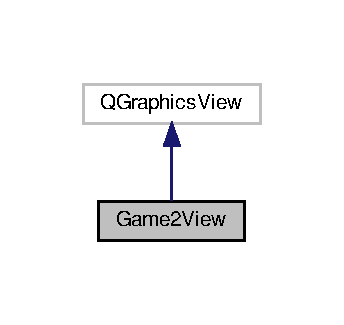
\includegraphics[width=165pt]{classGame2View__inherit__graph}
\end{center}
\end{figure}


Collaboration diagram for Game2\+View\+:
\nopagebreak
\begin{figure}[H]
\begin{center}
\leavevmode
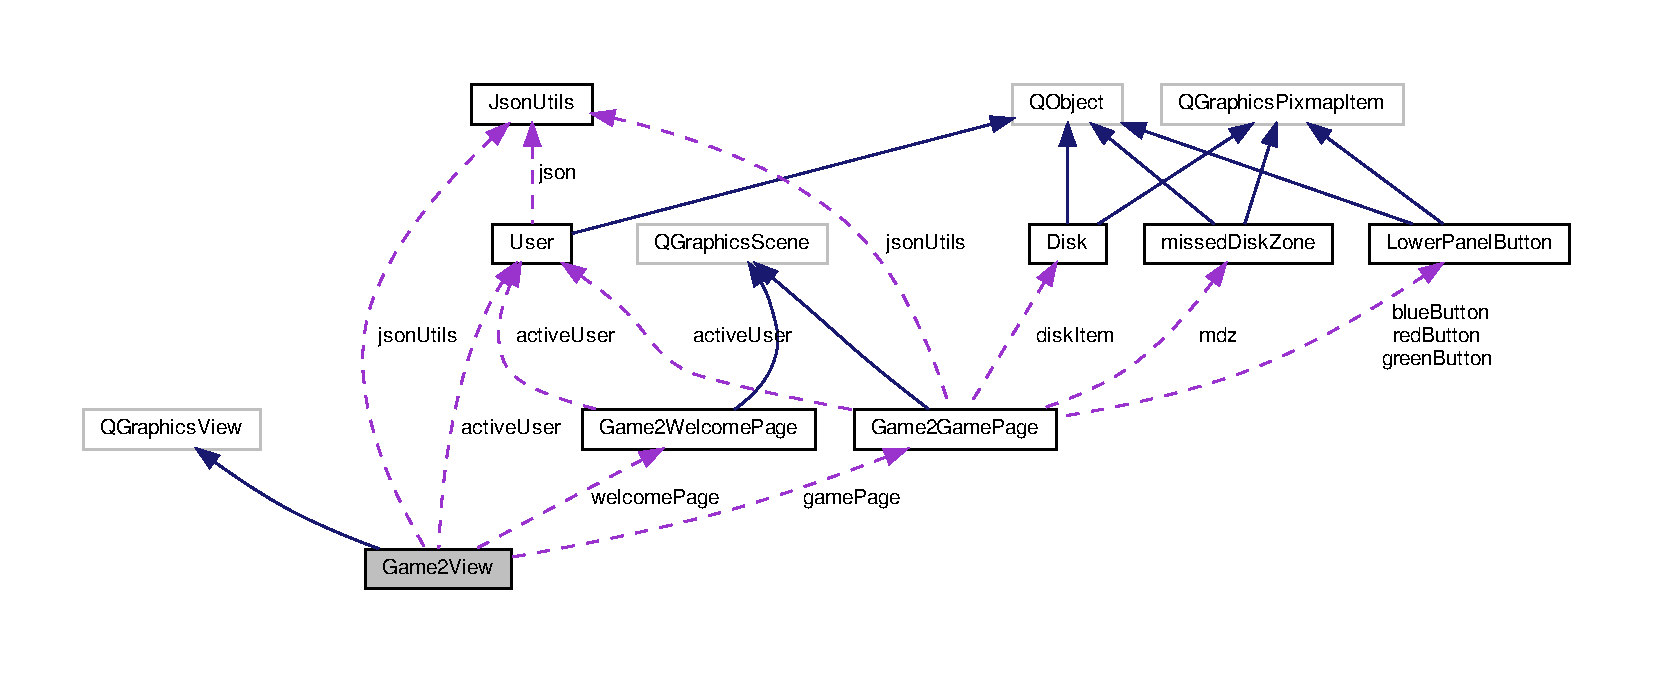
\includegraphics[width=350pt]{classGame2View__coll__graph}
\end{center}
\end{figure}
\subsection*{Public Slots}
\begin{DoxyCompactItemize}
\item 
\mbox{\Hypertarget{classGame2View_a0b81a7c2cb3223cd92d994e0909719c9}\label{classGame2View_a0b81a7c2cb3223cd92d994e0909719c9}} 
void \hyperlink{classGame2View_a0b81a7c2cb3223cd92d994e0909719c9}{start\+Game} ()
\begin{DoxyCompactList}\small\item\em \hyperlink{classGame2View_a0b81a7c2cb3223cd92d994e0909719c9}{Game2\+View\+::start\+Game}, is called to start the game. \end{DoxyCompactList}\item 
\mbox{\Hypertarget{classGame2View_a18957227e6e08549506c1f5e6628e71b}\label{classGame2View_a18957227e6e08549506c1f5e6628e71b}} 
void \hyperlink{classGame2View_a18957227e6e08549506c1f5e6628e71b}{go\+To\+Home} ()
\begin{DoxyCompactList}\small\item\em \hyperlink{classGame2View_a18957227e6e08549506c1f5e6628e71b}{Game2\+View\+::go\+To\+Home}, is called when home button is pressed, stops the game and takes the player back to the welcome page. \end{DoxyCompactList}\end{DoxyCompactItemize}
\subsection*{Public Member Functions}
\begin{DoxyCompactItemize}
\item 
\mbox{\Hypertarget{classGame2View_a14ea90578ed2a2ee3a4938dd4ca2c648}\label{classGame2View_a14ea90578ed2a2ee3a4938dd4ca2c648}} 
void \hyperlink{classGame2View_a14ea90578ed2a2ee3a4938dd4ca2c648}{key\+Press\+Event} (Q\+Key\+Event $\ast$event)
\begin{DoxyCompactList}\small\item\em \hyperlink{classGame2View_a14ea90578ed2a2ee3a4938dd4ca2c648}{Game2\+View\+::key\+Press\+Event}, is called when the arrow keys are pressed to delete the disks and add to the score. \end{DoxyCompactList}\item 
\mbox{\Hypertarget{classGame2View_a9ba086e311faddeed6a28cf9e727719c}\label{classGame2View_a9ba086e311faddeed6a28cf9e727719c}} 
void \hyperlink{classGame2View_a9ba086e311faddeed6a28cf9e727719c}{connect\+Buttons} ()
\begin{DoxyCompactList}\small\item\em \hyperlink{classGame2View_a9ba086e311faddeed6a28cf9e727719c}{Game2\+View\+::connect\+Buttons}, connects the buttons to the functions that need to be called when they are clicked. \end{DoxyCompactList}\end{DoxyCompactItemize}
\subsection*{Public Attributes}
\begin{DoxyCompactItemize}
\item 
\mbox{\Hypertarget{classGame2View_af6ff0b22ab9059944b9360619c20e4d9}\label{classGame2View_af6ff0b22ab9059944b9360619c20e4d9}} 
\hyperlink{classUser}{User} $\ast$ {\bfseries active\+User} = N\+U\+LL
\item 
\mbox{\Hypertarget{classGame2View_ad2418450777f817b67ff2b419d22de37}\label{classGame2View_ad2418450777f817b67ff2b419d22de37}} 
Q\+Graphics\+View $\ast$ {\bfseries app\+Main\+View}
\item 
\mbox{\Hypertarget{classGame2View_a34cd40d8efdb712c11a728f8ea58846e}\label{classGame2View_a34cd40d8efdb712c11a728f8ea58846e}} 
\hyperlink{classJsonUtils}{Json\+Utils} $\ast$ {\bfseries json\+Utils}
\item 
\mbox{\Hypertarget{classGame2View_a649d6baa095bd8c5137f048f6ff25fe3}\label{classGame2View_a649d6baa095bd8c5137f048f6ff25fe3}} 
\hyperlink{classGame2WelcomePage}{Game2\+Welcome\+Page} $\ast$ {\bfseries welcome\+Page}
\item 
\mbox{\Hypertarget{classGame2View_a464373379b7b9a087d7013c53c252ec9}\label{classGame2View_a464373379b7b9a087d7013c53c252ec9}} 
\hyperlink{classGame2GamePage}{Game2\+Game\+Page} $\ast$ {\bfseries game\+Page}
\end{DoxyCompactItemize}


The documentation for this class was generated from the following files\+:\begin{DoxyCompactItemize}
\item 
Game2-\/\+Shooting\+Discs/game2view.\+h\item 
Game2-\/\+Shooting\+Discs/game2view.\+cpp\end{DoxyCompactItemize}

\hypertarget{classGame2WelcomePage}{}\section{Game2\+Welcome\+Page Class Reference}
\label{classGame2WelcomePage}\index{Game2\+Welcome\+Page@{Game2\+Welcome\+Page}}


Inheritance diagram for Game2\+Welcome\+Page\+:
\nopagebreak
\begin{figure}[H]
\begin{center}
\leavevmode
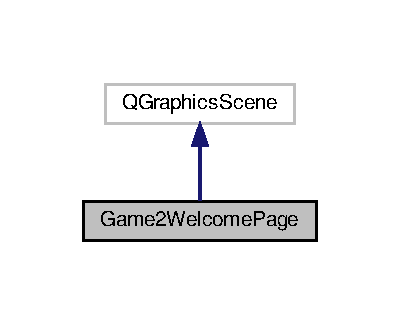
\includegraphics[width=192pt]{classGame2WelcomePage__inherit__graph}
\end{center}
\end{figure}


Collaboration diagram for Game2\+Welcome\+Page\+:
\nopagebreak
\begin{figure}[H]
\begin{center}
\leavevmode
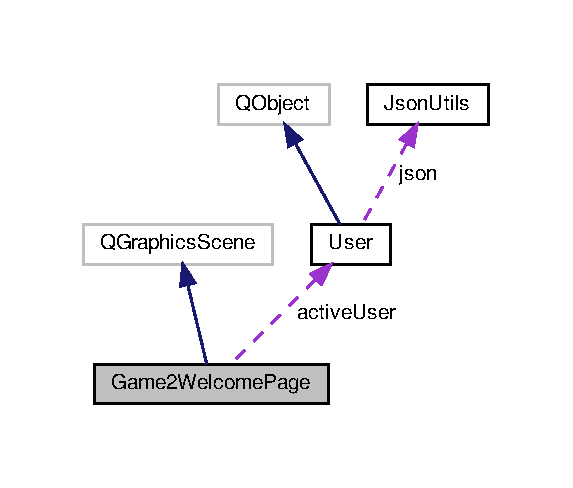
\includegraphics[width=275pt]{classGame2WelcomePage__coll__graph}
\end{center}
\end{figure}
\subsection*{Public Member Functions}
\begin{DoxyCompactItemize}
\item 
\mbox{\Hypertarget{classGame2WelcomePage_a25b5f78d9d26d51297edb5d897639ffd}\label{classGame2WelcomePage_a25b5f78d9d26d51297edb5d897639ffd}} 
void \hyperlink{classGame2WelcomePage_a25b5f78d9d26d51297edb5d897639ffd}{setup\+Scene} ()
\begin{DoxyCompactList}\small\item\em \hyperlink{classGame2GamePage_ab71efdf6cb71c97b5a2238949f0c95b7}{Game2\+Game\+Page\+::setup\+Scene}, sets up the welcome page instructions and widgets. \end{DoxyCompactList}\end{DoxyCompactItemize}
\subsection*{Public Attributes}
\begin{DoxyCompactItemize}
\item 
\mbox{\Hypertarget{classGame2WelcomePage_a1839c53ae10ec1b5dc2f158a74fff1ff}\label{classGame2WelcomePage_a1839c53ae10ec1b5dc2f158a74fff1ff}} 
\hyperlink{classUser}{User} $\ast$ {\bfseries active\+User} = N\+U\+LL
\item 
\mbox{\Hypertarget{classGame2WelcomePage_a6cb475e10f6095d72ca0bce9948222c4}\label{classGame2WelcomePage_a6cb475e10f6095d72ca0bce9948222c4}} 
Q\+Label $\ast$ {\bfseries game\+Name}
\item 
\mbox{\Hypertarget{classGame2WelcomePage_a4477b9e97fc0f815c84b1e9e6475e3ce}\label{classGame2WelcomePage_a4477b9e97fc0f815c84b1e9e6475e3ce}} 
Q\+Label $\ast$ {\bfseries game\+Insructions}
\item 
\mbox{\Hypertarget{classGame2WelcomePage_a8ae329cbb14582c73bcd03275b119fed}\label{classGame2WelcomePage_a8ae329cbb14582c73bcd03275b119fed}} 
Q\+Push\+Button $\ast$ {\bfseries play\+Game}
\end{DoxyCompactItemize}


The documentation for this class was generated from the following files\+:\begin{DoxyCompactItemize}
\item 
Game2-\/\+Shooting\+Discs/game2welcomepage.\+h\item 
Game2-\/\+Shooting\+Discs/game2welcomepage.\+cpp\end{DoxyCompactItemize}

\hypertarget{classJsonUtils}{}\section{Json\+Utils Class Reference}
\label{classJsonUtils}\index{Json\+Utils@{Json\+Utils}}
\subsection*{Public Member Functions}
\begin{DoxyCompactItemize}
\item 
void \hyperlink{classJsonUtils_a9626b00d2b338602731abac985a77063}{add\+User\+To\+Json} (Q\+Json\+Object user)
\begin{DoxyCompactList}\small\item\em Takes a newly created user and appends it to the users.\+json document. \end{DoxyCompactList}\item 
void \hyperlink{classJsonUtils_aa59b55bcdf1b0a9ab2726d1da6cf9eb8}{update\+Scores} (Q\+String username, Q\+Vector$<$ int $>$ scores, int highscore, int game\+Identifier)
\begin{DoxyCompactList}\small\item\em \hyperlink{classJsonUtils_aa59b55bcdf1b0a9ab2726d1da6cf9eb8}{Json\+Utils\+::update\+Scores}, Update the \hyperlink{classUser}{User} Scores in the Json object of the \hyperlink{classUser}{User}. \end{DoxyCompactList}\item 
Q\+Json\+Document \hyperlink{classJsonUtils_a119512273e8b9dc8ea46e88811479705}{get\+Json\+Document} ()
\begin{DoxyCompactList}\small\item\em Gets the Json\+Document of the file path. \end{DoxyCompactList}\item 
Q\+Json\+Object \hyperlink{classJsonUtils_ae71b2b3eeaf9d1d0a7dce02cec7684ea}{validate\+User} (Q\+String \&username, Q\+String \&password)
\begin{DoxyCompactList}\small\item\em Checks if a user who attempted to login has already signed up before. \end{DoxyCompactList}\item 
Q\+Json\+Value \hyperlink{classJsonUtils_ae1a169f74290c719847414f70d2cf970}{encode\+Profile\+Picture} (Q\+Pixmap \&p)
\begin{DoxyCompactList}\small\item\em \hyperlink{classJsonUtils_ae1a169f74290c719847414f70d2cf970}{Json\+Utils\+::encode\+Profile\+Picture}, Takes a picture, encodes it, and returns the corresponding hashed Q\+Json\+Value. \end{DoxyCompactList}\item 
Q\+Pixmap \hyperlink{classJsonUtils_aec5239b893c527428ed31a7ba05eba97}{decode\+Profile\+Picture} (Q\+Json\+Value pic)
\begin{DoxyCompactList}\small\item\em \hyperlink{classJsonUtils_aec5239b893c527428ed31a7ba05eba97}{Json\+Utils\+::decode\+Profile\+Picture}, Takes a Q\+Json\+Value corresponding to a picture, decodes it, and returns the corresponding Q\+Pixmap. \end{DoxyCompactList}\end{DoxyCompactItemize}
\subsection*{Public Attributes}
\begin{DoxyCompactItemize}
\item 
\mbox{\Hypertarget{classJsonUtils_a62ef956f6d79a2935be9fe199fc285b5}\label{classJsonUtils_a62ef956f6d79a2935be9fe199fc285b5}} 
Q\+String {\bfseries path\+To\+Json\+File}
\end{DoxyCompactItemize}


\subsection{Member Function Documentation}
\mbox{\Hypertarget{classJsonUtils_a9626b00d2b338602731abac985a77063}\label{classJsonUtils_a9626b00d2b338602731abac985a77063}} 
\index{Json\+Utils@{Json\+Utils}!add\+User\+To\+Json@{add\+User\+To\+Json}}
\index{add\+User\+To\+Json@{add\+User\+To\+Json}!Json\+Utils@{Json\+Utils}}
\subsubsection{\texorpdfstring{add\+User\+To\+Json()}{addUserToJson()}}
{\footnotesize\ttfamily void Json\+Utils\+::add\+User\+To\+Json (\begin{DoxyParamCaption}\item[{Q\+Json\+Object}]{user }\end{DoxyParamCaption})}



Takes a newly created user and appends it to the users.\+json document. 


\begin{DoxyParams}{Parameters}
{\em \hyperlink{classUser}{User}} & Object of type Q\+Json Object \\
\hline
\end{DoxyParams}
\mbox{\Hypertarget{classJsonUtils_aec5239b893c527428ed31a7ba05eba97}\label{classJsonUtils_aec5239b893c527428ed31a7ba05eba97}} 
\index{Json\+Utils@{Json\+Utils}!decode\+Profile\+Picture@{decode\+Profile\+Picture}}
\index{decode\+Profile\+Picture@{decode\+Profile\+Picture}!Json\+Utils@{Json\+Utils}}
\subsubsection{\texorpdfstring{decode\+Profile\+Picture()}{decodeProfilePicture()}}
{\footnotesize\ttfamily Q\+Pixmap Json\+Utils\+::decode\+Profile\+Picture (\begin{DoxyParamCaption}\item[{Q\+Json\+Value}]{pic }\end{DoxyParamCaption})}



\hyperlink{classJsonUtils_aec5239b893c527428ed31a7ba05eba97}{Json\+Utils\+::decode\+Profile\+Picture}, Takes a Q\+Json\+Value corresponding to a picture, decodes it, and returns the corresponding Q\+Pixmap. 


\begin{DoxyParams}{Parameters}
{\em pic} & \\
\hline
\end{DoxyParams}
\begin{DoxyReturn}{Returns}
Q\+Json\+Value for the decoded image 
\end{DoxyReturn}
\mbox{\Hypertarget{classJsonUtils_ae1a169f74290c719847414f70d2cf970}\label{classJsonUtils_ae1a169f74290c719847414f70d2cf970}} 
\index{Json\+Utils@{Json\+Utils}!encode\+Profile\+Picture@{encode\+Profile\+Picture}}
\index{encode\+Profile\+Picture@{encode\+Profile\+Picture}!Json\+Utils@{Json\+Utils}}
\subsubsection{\texorpdfstring{encode\+Profile\+Picture()}{encodeProfilePicture()}}
{\footnotesize\ttfamily Q\+Json\+Value Json\+Utils\+::encode\+Profile\+Picture (\begin{DoxyParamCaption}\item[{Q\+Pixmap \&}]{p }\end{DoxyParamCaption})}



\hyperlink{classJsonUtils_ae1a169f74290c719847414f70d2cf970}{Json\+Utils\+::encode\+Profile\+Picture}, Takes a picture, encodes it, and returns the corresponding hashed Q\+Json\+Value. 


\begin{DoxyParams}{Parameters}
{\em p,picture} & \\
\hline
\end{DoxyParams}
\begin{DoxyReturn}{Returns}
Q\+Json\+Value for the encoded image 
\end{DoxyReturn}
\mbox{\Hypertarget{classJsonUtils_a119512273e8b9dc8ea46e88811479705}\label{classJsonUtils_a119512273e8b9dc8ea46e88811479705}} 
\index{Json\+Utils@{Json\+Utils}!get\+Json\+Document@{get\+Json\+Document}}
\index{get\+Json\+Document@{get\+Json\+Document}!Json\+Utils@{Json\+Utils}}
\subsubsection{\texorpdfstring{get\+Json\+Document()}{getJsonDocument()}}
{\footnotesize\ttfamily Q\+Json\+Document Json\+Utils\+::get\+Json\+Document (\begin{DoxyParamCaption}{ }\end{DoxyParamCaption})}



Gets the Json\+Document of the file path. 

\begin{DoxyReturn}{Returns}
Q\+Json\+Document of the file path 
\end{DoxyReturn}
\mbox{\Hypertarget{classJsonUtils_aa59b55bcdf1b0a9ab2726d1da6cf9eb8}\label{classJsonUtils_aa59b55bcdf1b0a9ab2726d1da6cf9eb8}} 
\index{Json\+Utils@{Json\+Utils}!update\+Scores@{update\+Scores}}
\index{update\+Scores@{update\+Scores}!Json\+Utils@{Json\+Utils}}
\subsubsection{\texorpdfstring{update\+Scores()}{updateScores()}}
{\footnotesize\ttfamily void Json\+Utils\+::update\+Scores (\begin{DoxyParamCaption}\item[{Q\+String}]{username,  }\item[{Q\+Vector$<$ int $>$}]{scores,  }\item[{int}]{highscore,  }\item[{int}]{game\+Identifier }\end{DoxyParamCaption})}



\hyperlink{classJsonUtils_aa59b55bcdf1b0a9ab2726d1da6cf9eb8}{Json\+Utils\+::update\+Scores}, Update the \hyperlink{classUser}{User} Scores in the Json object of the \hyperlink{classUser}{User}. 


\begin{DoxyParams}{Parameters}
{\em username,username} & of \hyperlink{classUser}{User} \\
\hline
{\em scores,scores} & Arraylist of user \\
\hline
{\em highscore,User\textquotesingle{}s} & Highscore \\
\hline
{\em game\+Identifier,0} & for game1 and 1 for game2 \\
\hline
\end{DoxyParams}
\mbox{\Hypertarget{classJsonUtils_ae71b2b3eeaf9d1d0a7dce02cec7684ea}\label{classJsonUtils_ae71b2b3eeaf9d1d0a7dce02cec7684ea}} 
\index{Json\+Utils@{Json\+Utils}!validate\+User@{validate\+User}}
\index{validate\+User@{validate\+User}!Json\+Utils@{Json\+Utils}}
\subsubsection{\texorpdfstring{validate\+User()}{validateUser()}}
{\footnotesize\ttfamily Q\+Json\+Object Json\+Utils\+::validate\+User (\begin{DoxyParamCaption}\item[{Q\+String \&}]{username,  }\item[{Q\+String \&}]{password }\end{DoxyParamCaption})}



Checks if a user who attempted to login has already signed up before. 


\begin{DoxyParams}{Parameters}
{\em username,username} & of user \\
\hline
{\em password,password} & of user \\
\hline
\end{DoxyParams}
\begin{DoxyReturn}{Returns}
If the login was successful, returns the user as a Q\+Json\+Object.\+Else returns an empty Q\+J\+Son\+Object 
\end{DoxyReturn}


The documentation for this class was generated from the following files\+:\begin{DoxyCompactItemize}
\item 
Accounts\+\_\+\+Framework/jsonutils.\+h\item 
Accounts\+\_\+\+Framework/jsonutils.\+cpp\end{DoxyCompactItemize}

\hypertarget{classLandingPage}{}\section{Landing\+Page Class Reference}
\label{classLandingPage}\index{Landing\+Page@{Landing\+Page}}


Inheritance diagram for Landing\+Page\+:
\nopagebreak
\begin{figure}[H]
\begin{center}
\leavevmode
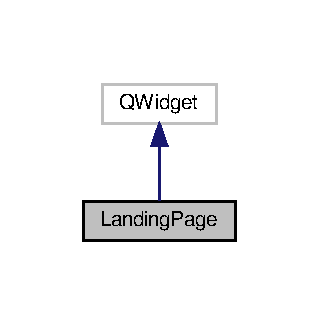
\includegraphics[width=153pt]{classLandingPage__inherit__graph}
\end{center}
\end{figure}


Collaboration diagram for Landing\+Page\+:
\nopagebreak
\begin{figure}[H]
\begin{center}
\leavevmode
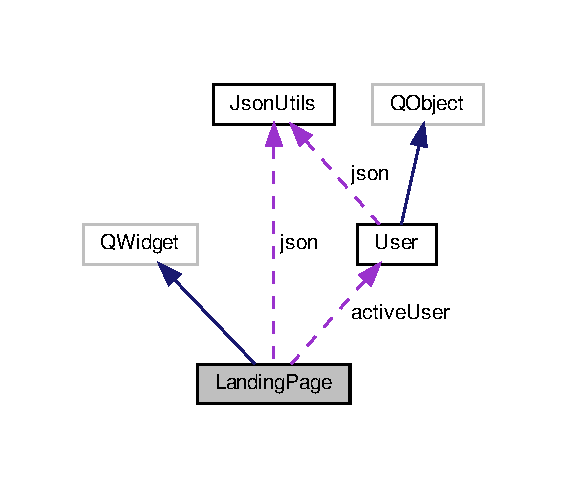
\includegraphics[width=272pt]{classLandingPage__coll__graph}
\end{center}
\end{figure}
\subsection*{Public Member Functions}
\begin{DoxyCompactItemize}
\item 
\hyperlink{classLandingPage_a44edf22c689206d962cfee656b50c68c}{Landing\+Page} (Q\+Widget $\ast$parent=nullptr)
\begin{DoxyCompactList}\small\item\em \hyperlink{classLandingPage_a44edf22c689206d962cfee656b50c68c}{Landing\+Page\+::\+Landing\+Page}, sets the geometry of all widgets and labels. Adds them to the scene. \end{DoxyCompactList}\end{DoxyCompactItemize}
\subsection*{Public Attributes}
\begin{DoxyCompactItemize}
\item 
\mbox{\Hypertarget{classLandingPage_ade505382a248c9dd438bebd05e4d97e2}\label{classLandingPage_ade505382a248c9dd438bebd05e4d97e2}} 
\hyperlink{classUser}{User} $\ast$ {\bfseries active\+User} = N\+U\+LL
\item 
\mbox{\Hypertarget{classLandingPage_af4e3bbbffaeac819e155b9469b8e7637}\label{classLandingPage_af4e3bbbffaeac819e155b9469b8e7637}} 
\hyperlink{classJsonUtils}{Json\+Utils} {\bfseries json}
\item 
\mbox{\Hypertarget{classLandingPage_a50c6ddfcb0b255fee3dd56fa4c9b824c}\label{classLandingPage_a50c6ddfcb0b255fee3dd56fa4c9b824c}} 
Q\+Label $\ast$ {\bfseries welcome\+Label}
\item 
\mbox{\Hypertarget{classLandingPage_acc3f6b67a349288c237fffad6320019b}\label{classLandingPage_acc3f6b67a349288c237fffad6320019b}} 
Q\+Label $\ast$ {\bfseries warning\+Label}
\item 
\mbox{\Hypertarget{classLandingPage_a40f3f068076aa792c022313c771efbba}\label{classLandingPage_a40f3f068076aa792c022313c771efbba}} 
Q\+Label $\ast$ {\bfseries user\+Name\+Label}
\item 
\mbox{\Hypertarget{classLandingPage_a745d6e547f5cded8fdf85f4ffebcf692}\label{classLandingPage_a745d6e547f5cded8fdf85f4ffebcf692}} 
Q\+Label $\ast$ {\bfseries password\+Label}
\item 
\mbox{\Hypertarget{classLandingPage_a12d650b1cda07a18943ed301e2458eca}\label{classLandingPage_a12d650b1cda07a18943ed301e2458eca}} 
Q\+Line\+Edit $\ast$ {\bfseries user\+Name\+Line\+Edit}
\item 
\mbox{\Hypertarget{classLandingPage_a8dcc6ee45a2e96aef191531562100aeb}\label{classLandingPage_a8dcc6ee45a2e96aef191531562100aeb}} 
Q\+Line\+Edit $\ast$ {\bfseries password\+Line\+Edit}
\item 
\mbox{\Hypertarget{classLandingPage_a79b9d94337a25c1c66245853586f0e49}\label{classLandingPage_a79b9d94337a25c1c66245853586f0e49}} 
Q\+Push\+Button $\ast$ {\bfseries sign\+In\+Push\+Button}
\item 
\mbox{\Hypertarget{classLandingPage_a770ca5552d0e19f3c88d889a9946fcd1}\label{classLandingPage_a770ca5552d0e19f3c88d889a9946fcd1}} 
Q\+Push\+Button $\ast$ {\bfseries sign\+Up\+Push\+Button}
\item 
\mbox{\Hypertarget{classLandingPage_ac006ddb5fbb6c397abdc6da03a6ff7c6}\label{classLandingPage_ac006ddb5fbb6c397abdc6da03a6ff7c6}} 
Q\+Push\+Button $\ast$ {\bfseries guest\+Push\+Button}
\item 
\mbox{\Hypertarget{classLandingPage_a75f2ed3f180997a8b8278b73af220f8a}\label{classLandingPage_a75f2ed3f180997a8b8278b73af220f8a}} 
Q\+Grid\+Layout $\ast$ {\bfseries grid\+Layout}
\item 
\mbox{\Hypertarget{classLandingPage_ad74571484af5f7eda5612036f59fc4c9}\label{classLandingPage_ad74571484af5f7eda5612036f59fc4c9}} 
Q\+V\+Box\+Layout $\ast$ {\bfseries vertical\+Layout}
\end{DoxyCompactItemize}


\subsection{Constructor \& Destructor Documentation}
\mbox{\Hypertarget{classLandingPage_a44edf22c689206d962cfee656b50c68c}\label{classLandingPage_a44edf22c689206d962cfee656b50c68c}} 
\index{Landing\+Page@{Landing\+Page}!Landing\+Page@{Landing\+Page}}
\index{Landing\+Page@{Landing\+Page}!Landing\+Page@{Landing\+Page}}
\subsubsection{\texorpdfstring{Landing\+Page()}{LandingPage()}}
{\footnotesize\ttfamily Landing\+Page\+::\+Landing\+Page (\begin{DoxyParamCaption}\item[{Q\+Widget $\ast$}]{parent = {\ttfamily nullptr} }\end{DoxyParamCaption})\hspace{0.3cm}{\ttfamily [explicit]}}



\hyperlink{classLandingPage_a44edf22c689206d962cfee656b50c68c}{Landing\+Page\+::\+Landing\+Page}, sets the geometry of all widgets and labels. Adds them to the scene. 


\begin{DoxyParams}{Parameters}
{\em parent} & \\
\hline
\end{DoxyParams}


The documentation for this class was generated from the following files\+:\begin{DoxyCompactItemize}
\item 
Accounts\+\_\+\+Framework/landingpage.\+h\item 
Accounts\+\_\+\+Framework/landingpage.\+cpp\end{DoxyCompactItemize}

\hypertarget{classLowerPanelButton}{}\section{Lower\+Panel\+Button Class Reference}
\label{classLowerPanelButton}\index{Lower\+Panel\+Button@{Lower\+Panel\+Button}}


Inheritance diagram for Lower\+Panel\+Button\+:
\nopagebreak
\begin{figure}[H]
\begin{center}
\leavevmode
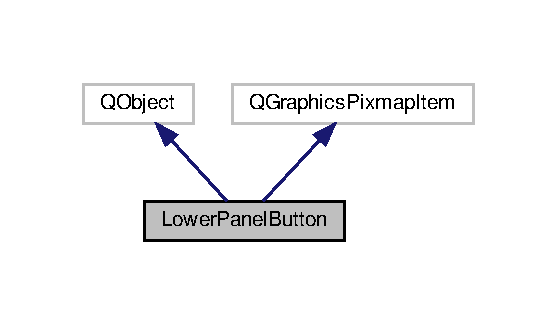
\includegraphics[width=268pt]{classLowerPanelButton__inherit__graph}
\end{center}
\end{figure}


Collaboration diagram for Lower\+Panel\+Button\+:
\nopagebreak
\begin{figure}[H]
\begin{center}
\leavevmode
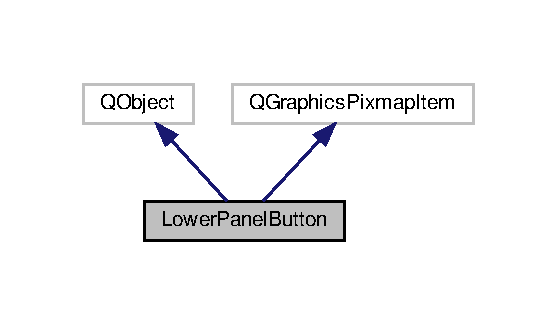
\includegraphics[width=268pt]{classLowerPanelButton__coll__graph}
\end{center}
\end{figure}
\subsection*{Public Member Functions}
\begin{DoxyCompactItemize}
\item 
\mbox{\Hypertarget{classLowerPanelButton_a01afac4f246ea833155b478fc374aba9}\label{classLowerPanelButton_a01afac4f246ea833155b478fc374aba9}} 
{\bfseries Lower\+Panel\+Button} (Q\+Object $\ast$parent=nullptr, int type=-\/1)
\end{DoxyCompactItemize}
\subsection*{Public Attributes}
\begin{DoxyCompactItemize}
\item 
\mbox{\Hypertarget{classLowerPanelButton_ad929b350b6b2629bf2d05eb9eea64c41}\label{classLowerPanelButton_ad929b350b6b2629bf2d05eb9eea64c41}} 
int {\bfseries type}
\end{DoxyCompactItemize}


The documentation for this class was generated from the following files\+:\begin{DoxyCompactItemize}
\item 
Game2-\/\+Shooting\+Discs/lowerpanelbutton.\+h\item 
Game2-\/\+Shooting\+Discs/lowerpanelbutton.\+cpp\end{DoxyCompactItemize}

\hypertarget{classmainPage}{}\section{main\+Page Class Reference}
\label{classmainPage}\index{main\+Page@{main\+Page}}


Inheritance diagram for main\+Page\+:
\nopagebreak
\begin{figure}[H]
\begin{center}
\leavevmode
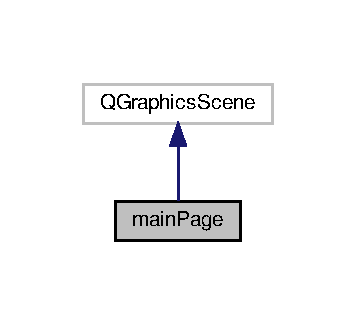
\includegraphics[width=171pt]{classmainPage__inherit__graph}
\end{center}
\end{figure}


Collaboration diagram for main\+Page\+:
\nopagebreak
\begin{figure}[H]
\begin{center}
\leavevmode
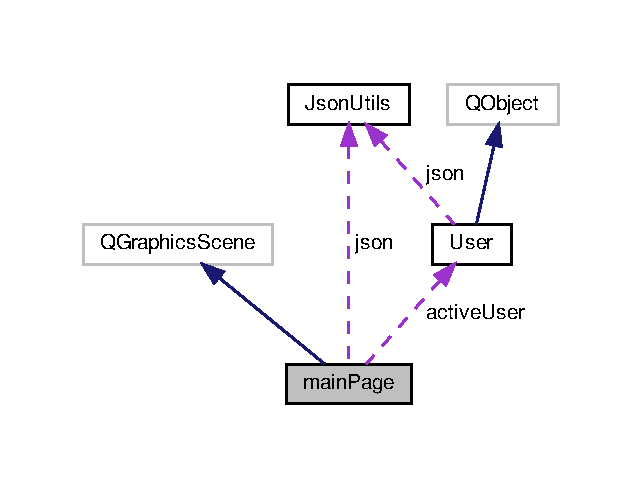
\includegraphics[width=308pt]{classmainPage__coll__graph}
\end{center}
\end{figure}
\subsection*{Public Member Functions}
\begin{DoxyCompactItemize}
\item 
\mbox{\Hypertarget{classmainPage_ad1718588c51fd343bc968bb7285b9788}\label{classmainPage_ad1718588c51fd343bc968bb7285b9788}} 
{\bfseries main\+Page} (Q\+Object $\ast$parent=nullptr)
\item 
\mbox{\Hypertarget{classmainPage_a95ca7745b5b82100f95af516c9fa21e2}\label{classmainPage_a95ca7745b5b82100f95af516c9fa21e2}} 
void \hyperlink{classmainPage_a95ca7745b5b82100f95af516c9fa21e2}{setup\+Game\+Logos} ()
\begin{DoxyCompactList}\small\item\em \hyperlink{classmainPage_a95ca7745b5b82100f95af516c9fa21e2}{main\+Page\+::setup\+Game\+Logos}, Sets the icons of the games in their corresponding place on the scene \end{DoxyCompactList}\item 
\mbox{\Hypertarget{classmainPage_a418bad8a789a1fdc183699ffd7758149}\label{classmainPage_a418bad8a789a1fdc183699ffd7758149}} 
void \hyperlink{classmainPage_a418bad8a789a1fdc183699ffd7758149}{setup\+Widget\+Locations} ()
\begin{DoxyCompactList}\small\item\em \hyperlink{classmainPage_a418bad8a789a1fdc183699ffd7758149}{main\+Page\+::setup\+Widget\+Locations}, Sets the geometry of the widgets \end{DoxyCompactList}\item 
\mbox{\Hypertarget{classmainPage_a6568ab3ff55a0004a211e0d398d99e71}\label{classmainPage_a6568ab3ff55a0004a211e0d398d99e71}} 
void \hyperlink{classmainPage_a6568ab3ff55a0004a211e0d398d99e71}{add\+Profile\+Picture} ()
\begin{DoxyCompactList}\small\item\em \hyperlink{classmainPage_a6568ab3ff55a0004a211e0d398d99e71}{main\+Page\+::add\+Profile\+Picture}, Decodes a user\textquotesingle{}s profile picture from a Q\+Json\+Value into a Q\+Pixmap. Sets the Pixmap p to the corresponding profile pic location on the scene \end{DoxyCompactList}\item 
\mbox{\Hypertarget{classmainPage_a5a1a5829cf997a8820ce25f3bc7826bf}\label{classmainPage_a5a1a5829cf997a8820ce25f3bc7826bf}} 
void \hyperlink{classmainPage_a5a1a5829cf997a8820ce25f3bc7826bf}{adjust\+Label\+Appearance} ()
\begin{DoxyCompactList}\small\item\em \hyperlink{classmainPage_a5a1a5829cf997a8820ce25f3bc7826bf}{main\+Page\+::adjust\+Label\+Appearance}, Function used to fix Labels. \end{DoxyCompactList}\item 
\mbox{\Hypertarget{classmainPage_abdede759b961f036fc1414fdfa784304}\label{classmainPage_abdede759b961f036fc1414fdfa784304}} 
void \hyperlink{classmainPage_abdede759b961f036fc1414fdfa784304}{fill\+Scene} ()
\begin{DoxyCompactList}\small\item\em \hyperlink{classmainPage_abdede759b961f036fc1414fdfa784304}{main\+Page\+::fill\+Scene}, Function Used to fill the Scene \end{DoxyCompactList}\item 
\mbox{\Hypertarget{classmainPage_aba3333bfeaa901530d9a832793ef5ca6}\label{classmainPage_aba3333bfeaa901530d9a832793ef5ca6}} 
void \hyperlink{classmainPage_aba3333bfeaa901530d9a832793ef5ca6}{update\+Scores} ()
\begin{DoxyCompactList}\small\item\em \hyperlink{classmainPage_aba3333bfeaa901530d9a832793ef5ca6}{main\+Page\+::update\+Scores}, Displays a user\textquotesingle{}s scores to the scene for each corresponding game \end{DoxyCompactList}\item 
\mbox{\Hypertarget{classmainPage_a43bd86b96287348d8ae5ec3368ecd92f}\label{classmainPage_a43bd86b96287348d8ae5ec3368ecd92f}} 
void \hyperlink{classmainPage_a43bd86b96287348d8ae5ec3368ecd92f}{clear\+Page} ()
\begin{DoxyCompactList}\small\item\em \hyperlink{classmainPage_a43bd86b96287348d8ae5ec3368ecd92f}{main\+Page\+::clear\+Page} Called when we need to go to the maingview Cleans all widgets in order to prepare for another user to login/signup \end{DoxyCompactList}\item 
\mbox{\Hypertarget{classmainPage_a36278cdd4e00b6fc0d5fe6ab20289a71}\label{classmainPage_a36278cdd4e00b6fc0d5fe6ab20289a71}} 
void \hyperlink{classmainPage_a36278cdd4e00b6fc0d5fe6ab20289a71}{set\+Flag} ()
\begin{DoxyCompactList}\small\item\em \hyperlink{classmainPage_a36278cdd4e00b6fc0d5fe6ab20289a71}{main\+Page\+::set\+Flag}, sets the flag for corresponding active user \end{DoxyCompactList}\end{DoxyCompactItemize}
\subsection*{Public Attributes}
\begin{DoxyCompactItemize}
\item 
\mbox{\Hypertarget{classmainPage_a09746ec017c3674d4cf6070d67878c5c}\label{classmainPage_a09746ec017c3674d4cf6070d67878c5c}} 
\hyperlink{classUser}{User} $\ast$ {\bfseries active\+User} = N\+U\+LL
\item 
\mbox{\Hypertarget{classmainPage_ad8aa4ec26116fc65f0c1fbdfc8f1c46a}\label{classmainPage_ad8aa4ec26116fc65f0c1fbdfc8f1c46a}} 
\hyperlink{classJsonUtils}{Json\+Utils} {\bfseries json}
\item 
\mbox{\Hypertarget{classmainPage_afba58f3009e3572b8538ec9b5091d3e2}\label{classmainPage_afba58f3009e3572b8538ec9b5091d3e2}} 
Q\+Label $\ast$ {\bfseries welcomeL}
\item 
\mbox{\Hypertarget{classmainPage_af4c776e295e005ce92db4ab2ad43b351}\label{classmainPage_af4c776e295e005ce92db4ab2ad43b351}} 
Q\+Label $\ast$ {\bfseries dateL}
\item 
\mbox{\Hypertarget{classmainPage_a8ded2dbb886faf41e7868c4e31d025e7}\label{classmainPage_a8ded2dbb886faf41e7868c4e31d025e7}} 
Q\+Graphics\+Pixmap\+Item $\ast$ {\bfseries game1\+Logo}
\item 
\mbox{\Hypertarget{classmainPage_a99262834603fa2a5286a4cc8eca69825}\label{classmainPage_a99262834603fa2a5286a4cc8eca69825}} 
Q\+Graphics\+Pixmap\+Item $\ast$ {\bfseries game2\+Logo}
\item 
\mbox{\Hypertarget{classmainPage_a81b4792c666b46bc47ae64d18292d80e}\label{classmainPage_a81b4792c666b46bc47ae64d18292d80e}} 
Q\+Graphics\+Pixmap\+Item $\ast$ {\bfseries user\+Profile\+Picture}
\item 
\mbox{\Hypertarget{classmainPage_ae2ae1e7d6cc2f465d539d9e7e73314f2}\label{classmainPage_ae2ae1e7d6cc2f465d539d9e7e73314f2}} 
Q\+Graphics\+Pixmap\+Item $\ast$ {\bfseries flag}
\item 
\mbox{\Hypertarget{classmainPage_a29b403e262009f83281f752eb6a91e62}\label{classmainPage_a29b403e262009f83281f752eb6a91e62}} 
Q\+Push\+Button $\ast$ {\bfseries game1B}
\item 
\mbox{\Hypertarget{classmainPage_a83a8da3a7de1fcef49732ce7cef07757}\label{classmainPage_a83a8da3a7de1fcef49732ce7cef07757}} 
Q\+Push\+Button $\ast$ {\bfseries game2B}
\item 
\mbox{\Hypertarget{classmainPage_a6b60c5103a4ffa5c3de03d8cfe22b5b5}\label{classmainPage_a6b60c5103a4ffa5c3de03d8cfe22b5b5}} 
Q\+Push\+Button $\ast$ {\bfseries homeB}
\item 
\mbox{\Hypertarget{classmainPage_a4ea215b0dd97ccaaeeecbb3e796fb7e1}\label{classmainPage_a4ea215b0dd97ccaaeeecbb3e796fb7e1}} 
Q\+Label $\ast$ {\bfseries game1\+Scores}
\item 
\mbox{\Hypertarget{classmainPage_a9469c2ef1da114595a159acb78008316}\label{classmainPage_a9469c2ef1da114595a159acb78008316}} 
Q\+Label $\ast$ {\bfseries game2\+Scores}
\end{DoxyCompactItemize}


The documentation for this class was generated from the following files\+:\begin{DoxyCompactItemize}
\item 
Accounts\+\_\+\+Framework/mainpage.\+h\item 
Accounts\+\_\+\+Framework/mainpage.\+cpp\end{DoxyCompactItemize}

\hypertarget{classmissedDiskZone}{}\section{missed\+Disk\+Zone Class Reference}
\label{classmissedDiskZone}\index{missed\+Disk\+Zone@{missed\+Disk\+Zone}}


Inheritance diagram for missed\+Disk\+Zone\+:
\nopagebreak
\begin{figure}[H]
\begin{center}
\leavevmode
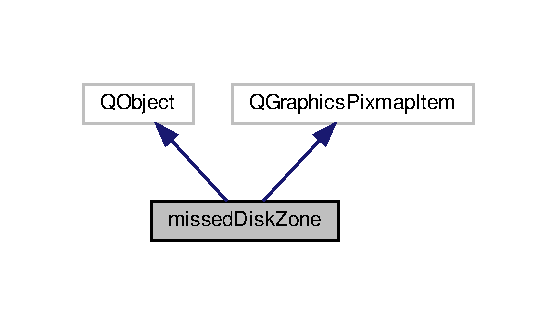
\includegraphics[width=268pt]{classmissedDiskZone__inherit__graph}
\end{center}
\end{figure}


Collaboration diagram for missed\+Disk\+Zone\+:
\nopagebreak
\begin{figure}[H]
\begin{center}
\leavevmode
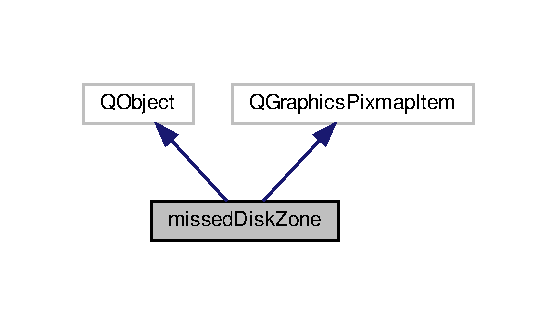
\includegraphics[width=268pt]{classmissedDiskZone__coll__graph}
\end{center}
\end{figure}
\subsection*{Public Member Functions}
\begin{DoxyCompactItemize}
\item 
\mbox{\Hypertarget{classmissedDiskZone_abb6e03300bfbb094d450914e1555db33}\label{classmissedDiskZone_abb6e03300bfbb094d450914e1555db33}} 
{\bfseries missed\+Disk\+Zone} (Q\+Object $\ast$parent=nullptr)
\end{DoxyCompactItemize}


The documentation for this class was generated from the following files\+:\begin{DoxyCompactItemize}
\item 
Game2-\/\+Shooting\+Discs/misseddiskzone.\+h\item 
Game2-\/\+Shooting\+Discs/misseddiskzone.\+cpp\end{DoxyCompactItemize}

\hypertarget{classQuestionObj}{}\section{Question\+Obj Class Reference}
\label{classQuestionObj}\index{Question\+Obj@{Question\+Obj}}


Inheritance diagram for Question\+Obj\+:
\nopagebreak
\begin{figure}[H]
\begin{center}
\leavevmode
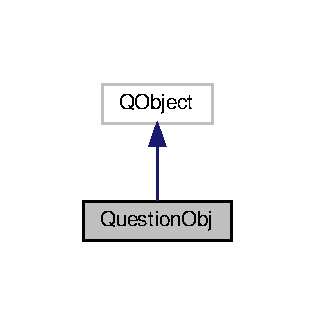
\includegraphics[width=151pt]{classQuestionObj__inherit__graph}
\end{center}
\end{figure}


Collaboration diagram for Question\+Obj\+:
\nopagebreak
\begin{figure}[H]
\begin{center}
\leavevmode
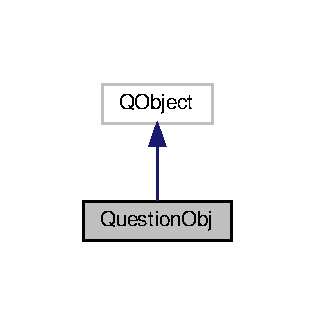
\includegraphics[width=151pt]{classQuestionObj__coll__graph}
\end{center}
\end{figure}
\subsection*{Public Member Functions}
\begin{DoxyCompactItemize}
\item 
\hyperlink{classQuestionObj_a6bdcb5f15f07cd5552597e3b03408ef2}{Question\+Obj} (Q\+Object $\ast$parent=nullptr)
\begin{DoxyCompactList}\small\item\em \hyperlink{classQuestionObj_a6bdcb5f15f07cd5552597e3b03408ef2}{Question\+Obj\+::\+Question\+Obj}, initializes a question object randomly. \end{DoxyCompactList}\item 
\hyperlink{classQuestionObj_a32bd699d1cdea35e8d2db5fd1c329479}{Question\+Obj} (Q\+Json\+Object json\+Question)
\begin{DoxyCompactList}\small\item\em \hyperlink{classQuestionObj_a6bdcb5f15f07cd5552597e3b03408ef2}{Question\+Obj\+::\+Question\+Obj}, returns a question object from a json input. \end{DoxyCompactList}\item 
Q\+Json\+Object \hyperlink{classQuestionObj_a0211af0ca0084c025f5793c27a83f172}{get\+Random\+Question\+From\+Json\+Document} ()
\begin{DoxyCompactList}\small\item\em \hyperlink{classQuestionObj_a0211af0ca0084c025f5793c27a83f172}{Question\+Obj\+::get\+Random\+Question\+From\+Json\+Document}, chooses a question by random from the Json document containing questions. \end{DoxyCompactList}\end{DoxyCompactItemize}
\subsection*{Public Attributes}
\begin{DoxyCompactItemize}
\item 
\mbox{\Hypertarget{classQuestionObj_a15696c2ae2f9b7ee5bca14d17b844c6f}\label{classQuestionObj_a15696c2ae2f9b7ee5bca14d17b844c6f}} 
Q\+String {\bfseries question}
\item 
\mbox{\Hypertarget{classQuestionObj_a2d37f7f7d2aa7beed70ac10ac4d9b926}\label{classQuestionObj_a2d37f7f7d2aa7beed70ac10ac4d9b926}} 
Q\+String {\bfseries true\+Answer}
\item 
\mbox{\Hypertarget{classQuestionObj_a329dcfdd9884aa21695fb0d791abf8e5}\label{classQuestionObj_a329dcfdd9884aa21695fb0d791abf8e5}} 
Q\+String {\bfseries false\+Answer}
\end{DoxyCompactItemize}


\subsection{Constructor \& Destructor Documentation}
\mbox{\Hypertarget{classQuestionObj_a6bdcb5f15f07cd5552597e3b03408ef2}\label{classQuestionObj_a6bdcb5f15f07cd5552597e3b03408ef2}} 
\index{Question\+Obj@{Question\+Obj}!Question\+Obj@{Question\+Obj}}
\index{Question\+Obj@{Question\+Obj}!Question\+Obj@{Question\+Obj}}
\subsubsection{\texorpdfstring{Question\+Obj()}{QuestionObj()}\hspace{0.1cm}{\footnotesize\ttfamily [1/2]}}
{\footnotesize\ttfamily Question\+Obj\+::\+Question\+Obj (\begin{DoxyParamCaption}\item[{Q\+Object $\ast$}]{parent = {\ttfamily nullptr} }\end{DoxyParamCaption})\hspace{0.3cm}{\ttfamily [explicit]}}



\hyperlink{classQuestionObj_a6bdcb5f15f07cd5552597e3b03408ef2}{Question\+Obj\+::\+Question\+Obj}, initializes a question object randomly. 


\begin{DoxyParams}{Parameters}
{\em parent} & \\
\hline
\end{DoxyParams}
\mbox{\Hypertarget{classQuestionObj_a32bd699d1cdea35e8d2db5fd1c329479}\label{classQuestionObj_a32bd699d1cdea35e8d2db5fd1c329479}} 
\index{Question\+Obj@{Question\+Obj}!Question\+Obj@{Question\+Obj}}
\index{Question\+Obj@{Question\+Obj}!Question\+Obj@{Question\+Obj}}
\subsubsection{\texorpdfstring{Question\+Obj()}{QuestionObj()}\hspace{0.1cm}{\footnotesize\ttfamily [2/2]}}
{\footnotesize\ttfamily Question\+Obj\+::\+Question\+Obj (\begin{DoxyParamCaption}\item[{Q\+Json\+Object}]{json\+Question }\end{DoxyParamCaption})\hspace{0.3cm}{\ttfamily [explicit]}}



\hyperlink{classQuestionObj_a6bdcb5f15f07cd5552597e3b03408ef2}{Question\+Obj\+::\+Question\+Obj}, returns a question object from a json input. 


\begin{DoxyParams}{Parameters}
{\em json\+Question,question} & read fron json file \\
\hline
\end{DoxyParams}


\subsection{Member Function Documentation}
\mbox{\Hypertarget{classQuestionObj_a0211af0ca0084c025f5793c27a83f172}\label{classQuestionObj_a0211af0ca0084c025f5793c27a83f172}} 
\index{Question\+Obj@{Question\+Obj}!get\+Random\+Question\+From\+Json\+Document@{get\+Random\+Question\+From\+Json\+Document}}
\index{get\+Random\+Question\+From\+Json\+Document@{get\+Random\+Question\+From\+Json\+Document}!Question\+Obj@{Question\+Obj}}
\subsubsection{\texorpdfstring{get\+Random\+Question\+From\+Json\+Document()}{getRandomQuestionFromJsonDocument()}}
{\footnotesize\ttfamily Q\+Json\+Object Question\+Obj\+::get\+Random\+Question\+From\+Json\+Document (\begin{DoxyParamCaption}{ }\end{DoxyParamCaption})}



\hyperlink{classQuestionObj_a0211af0ca0084c025f5793c27a83f172}{Question\+Obj\+::get\+Random\+Question\+From\+Json\+Document}, chooses a question by random from the Json document containing questions. 

\begin{DoxyReturn}{Returns}
question of type question\+Obj 
\end{DoxyReturn}


The documentation for this class was generated from the following files\+:\begin{DoxyCompactItemize}
\item 
Game1-\/\+Battle\+Ship/questionobj.\+h\item 
Game1-\/\+Battle\+Ship/questionobj.\+cpp\end{DoxyCompactItemize}

\hypertarget{classQuestionPage}{}\section{Question\+Page Class Reference}
\label{classQuestionPage}\index{Question\+Page@{Question\+Page}}


Inheritance diagram for Question\+Page\+:
\nopagebreak
\begin{figure}[H]
\begin{center}
\leavevmode
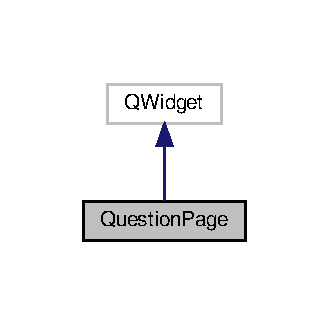
\includegraphics[width=158pt]{classQuestionPage__inherit__graph}
\end{center}
\end{figure}


Collaboration diagram for Question\+Page\+:
\nopagebreak
\begin{figure}[H]
\begin{center}
\leavevmode
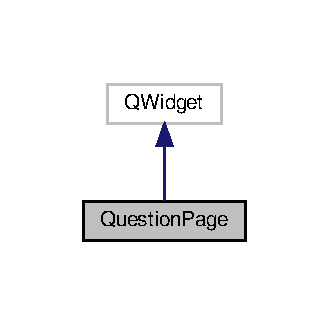
\includegraphics[width=158pt]{classQuestionPage__coll__graph}
\end{center}
\end{figure}
\subsection*{Public Member Functions}
\begin{DoxyCompactItemize}
\item 
\mbox{\Hypertarget{classQuestionPage_a0e5942772dea0003205663676b1b667c}\label{classQuestionPage_a0e5942772dea0003205663676b1b667c}} 
{\bfseries Question\+Page} (Q\+Widget $\ast$parent=nullptr)
\item 
\mbox{\Hypertarget{classQuestionPage_ac2485d12691429ffd6c5a998a1f36865}\label{classQuestionPage_ac2485d12691429ffd6c5a998a1f36865}} 
void \hyperlink{classQuestionPage_ac2485d12691429ffd6c5a998a1f36865}{generate\+Question} ()
\begin{DoxyCompactList}\small\item\em \hyperlink{classQuestionPage_ac2485d12691429ffd6c5a998a1f36865}{Question\+Page\+::generate\+Question}, generates a new question object and updates the question page accordingly. \end{DoxyCompactList}\end{DoxyCompactItemize}
\subsection*{Public Attributes}
\begin{DoxyCompactItemize}
\item 
\mbox{\Hypertarget{classQuestionPage_a76b4abc3747e379085607ef98c0b6907}\label{classQuestionPage_a76b4abc3747e379085607ef98c0b6907}} 
Q\+Label $\ast$ {\bfseries questionL}
\item 
\mbox{\Hypertarget{classQuestionPage_a57b3b9a39a380b0b61ac28106c813fa1}\label{classQuestionPage_a57b3b9a39a380b0b61ac28106c813fa1}} 
Q\+Push\+Button $\ast$ {\bfseries correct\+Answer\+PB}
\item 
\mbox{\Hypertarget{classQuestionPage_aed1e1c5159986ade73742ee79e0cb2b3}\label{classQuestionPage_aed1e1c5159986ade73742ee79e0cb2b3}} 
Q\+Push\+Button $\ast$ {\bfseries wrong\+Answer\+PB}
\item 
\mbox{\Hypertarget{classQuestionPage_a3bb573fd39499fad91b1bba794889b78}\label{classQuestionPage_a3bb573fd39499fad91b1bba794889b78}} 
Q\+V\+Box\+Layout $\ast$ {\bfseries vlayout}
\end{DoxyCompactItemize}


The documentation for this class was generated from the following files\+:\begin{DoxyCompactItemize}
\item 
Game1-\/\+Battle\+Ship/questionpage.\+h\item 
Game1-\/\+Battle\+Ship/questionpage.\+cpp\end{DoxyCompactItemize}

\hypertarget{classSignupPage}{}\section{Signup\+Page Class Reference}
\label{classSignupPage}\index{Signup\+Page@{Signup\+Page}}


Inheritance diagram for Signup\+Page\+:
\nopagebreak
\begin{figure}[H]
\begin{center}
\leavevmode
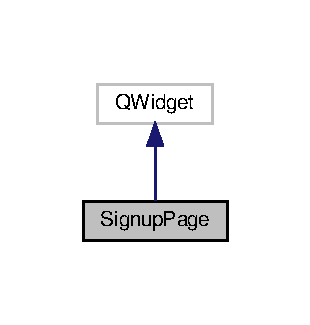
\includegraphics[width=149pt]{classSignupPage__inherit__graph}
\end{center}
\end{figure}


Collaboration diagram for Signup\+Page\+:
\nopagebreak
\begin{figure}[H]
\begin{center}
\leavevmode
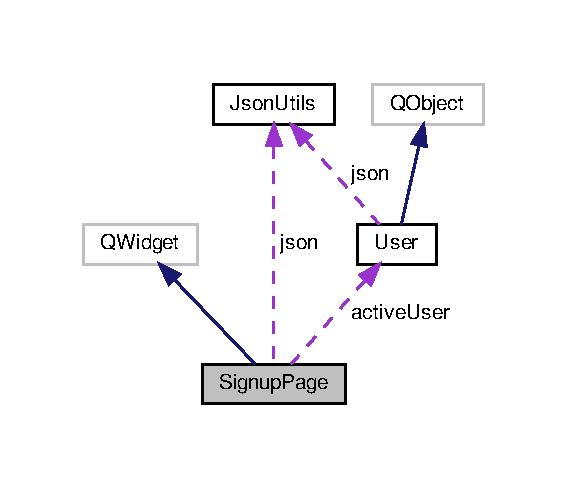
\includegraphics[width=272pt]{classSignupPage__coll__graph}
\end{center}
\end{figure}
\subsection*{Public Slots}
\begin{DoxyCompactItemize}
\item 
\mbox{\Hypertarget{classSignupPage_a9b2f3559ecf002b3a35c73348e0d7e81}\label{classSignupPage_a9b2f3559ecf002b3a35c73348e0d7e81}} 
void \hyperlink{classSignupPage_a9b2f3559ecf002b3a35c73348e0d7e81}{add\+User} ()
\begin{DoxyCompactList}\small\item\em \hyperlink{classSignupPage_a9b2f3559ecf002b3a35c73348e0d7e81}{Signup\+Page\+::add\+User} Called whenever the signup button is pressed calls \hyperlink{classSignupPage_ac6f433285ca77bcfa6bae1d3b37cd5b5}{create\+User()} in order to check all necessary conditions before adding a new user to the users.\+json file if \hyperlink{classSignupPage_ac6f433285ca77bcfa6bae1d3b37cd5b5}{create\+User()} returned a user, set\+User() appends it to users.\+json. \end{DoxyCompactList}\item 
void \hyperlink{classSignupPage_a53027011ed8c2cf3e098468269bee0db}{browse\+Image} ()
\begin{DoxyCompactList}\small\item\em \hyperlink{classSignupPage_a53027011ed8c2cf3e098468269bee0db}{Signup\+Page\+::browse\+Image}. \end{DoxyCompactList}\end{DoxyCompactItemize}
\subsection*{Public Member Functions}
\begin{DoxyCompactItemize}
\item 
\mbox{\Hypertarget{classSignupPage_af41bce1fd7c7e7f6b78e7dd0e790f1c5}\label{classSignupPage_af41bce1fd7c7e7f6b78e7dd0e790f1c5}} 
{\bfseries Signup\+Page} (Q\+Widget $\ast$parent=nullptr)
\item 
bool \hyperlink{classSignupPage_afe8c63473a69b4763c1cbe9aaafbe895}{check\+Password} (Q\+String password)
\begin{DoxyCompactList}\small\item\em \hyperlink{classSignupPage_afe8c63473a69b4763c1cbe9aaafbe895}{Signup\+Page\+::check\+Password}, Checks if a password is valid, of size at least 4 and have special chars. \end{DoxyCompactList}\item 
\hyperlink{classUser}{User} $\ast$ \hyperlink{classSignupPage_ac6f433285ca77bcfa6bae1d3b37cd5b5}{create\+User} ()
\begin{DoxyCompactList}\small\item\em \hyperlink{classSignupPage_ac6f433285ca77bcfa6bae1d3b37cd5b5}{Signup\+Page\+::create\+User}, Reads the input from the widgets and attemps to create a new user. \end{DoxyCompactList}\item 
\mbox{\Hypertarget{classSignupPage_ac686137b3a91a6d56fa016317108d74e}\label{classSignupPage_ac686137b3a91a6d56fa016317108d74e}} 
void \hyperlink{classSignupPage_ac686137b3a91a6d56fa016317108d74e}{clear\+Page} ()
\begin{DoxyCompactList}\small\item\em \hyperlink{classSignupPage_ac686137b3a91a6d56fa016317108d74e}{Signup\+Page\+::clear\+Page}, this methods resets all the widgets that took user input. \end{DoxyCompactList}\item 
\mbox{\Hypertarget{classSignupPage_afed84bf2953680930fbf70c1d16b3882}\label{classSignupPage_afed84bf2953680930fbf70c1d16b3882}} 
void \hyperlink{classSignupPage_afed84bf2953680930fbf70c1d16b3882}{setup\+Widgets} ()
\begin{DoxyCompactList}\small\item\em \hyperlink{classSignupPage_afed84bf2953680930fbf70c1d16b3882}{Signup\+Page\+::setup\+Widgets} Sets the geometry of the widgets. \end{DoxyCompactList}\end{DoxyCompactItemize}
\subsection*{Public Attributes}
\begin{DoxyCompactItemize}
\item 
\mbox{\Hypertarget{classSignupPage_abe5b85695bd3875f897bb68c2ee4a863}\label{classSignupPage_abe5b85695bd3875f897bb68c2ee4a863}} 
\hyperlink{classUser}{User} $\ast$ {\bfseries active\+User} = N\+U\+LL
\item 
\mbox{\Hypertarget{classSignupPage_a236ecc9b13706daeb87bfaf67f772952}\label{classSignupPage_a236ecc9b13706daeb87bfaf67f772952}} 
\hyperlink{classJsonUtils}{Json\+Utils} {\bfseries json}
\item 
\mbox{\Hypertarget{classSignupPage_a193020d33d7b35806f868780022aecba}\label{classSignupPage_a193020d33d7b35806f868780022aecba}} 
Q\+Label $\ast$ {\bfseries headerL}
\item 
\mbox{\Hypertarget{classSignupPage_a030f14d4cd531e4d575c6edbfc6c283d}\label{classSignupPage_a030f14d4cd531e4d575c6edbfc6c283d}} 
Q\+Label $\ast$ {\bfseries warningL}
\item 
\mbox{\Hypertarget{classSignupPage_a9c5b23d7abe45d44ead6f0e45b07083c}\label{classSignupPage_a9c5b23d7abe45d44ead6f0e45b07083c}} 
Q\+Label $\ast$ {\bfseries Sign\+In\+PromptL}
\item 
\mbox{\Hypertarget{classSignupPage_a103ee8978a998cfb9ae7ab55ef830478}\label{classSignupPage_a103ee8978a998cfb9ae7ab55ef830478}} 
Q\+Line\+Edit $\ast$ {\bfseries first\+Name\+LE}
\item 
\mbox{\Hypertarget{classSignupPage_a74ab0d823f652c56e14a3b3ae482f655}\label{classSignupPage_a74ab0d823f652c56e14a3b3ae482f655}} 
Q\+Line\+Edit $\ast$ {\bfseries last\+Name\+LE}
\item 
\mbox{\Hypertarget{classSignupPage_a44d748829a851eee9506750bfb127136}\label{classSignupPage_a44d748829a851eee9506750bfb127136}} 
Q\+Line\+Edit $\ast$ {\bfseries username\+LE}
\item 
\mbox{\Hypertarget{classSignupPage_af66076d8e5d0b6183e5bceccce4a57fc}\label{classSignupPage_af66076d8e5d0b6183e5bceccce4a57fc}} 
Q\+Line\+Edit $\ast$ {\bfseries password\+LE}
\item 
\mbox{\Hypertarget{classSignupPage_a514a50dd28266610eb74e41cdd6fd22c}\label{classSignupPage_a514a50dd28266610eb74e41cdd6fd22c}} 
Q\+Line\+Edit $\ast$ {\bfseries confirm\+Password\+LE}
\item 
\mbox{\Hypertarget{classSignupPage_a3b963d8ca9ca3450be0cf3e068f67b74}\label{classSignupPage_a3b963d8ca9ca3450be0cf3e068f67b74}} 
Q\+Line\+Edit $\ast$ {\bfseries phone\+Number\+LE}
\item 
\mbox{\Hypertarget{classSignupPage_a89113fdb187da73dcce9597032cdbe73}\label{classSignupPage_a89113fdb187da73dcce9597032cdbe73}} 
Q\+Spin\+Box $\ast$ {\bfseries day\+SB}
\item 
\mbox{\Hypertarget{classSignupPage_a42968b0dad7e3bfe2a1f5bb6fc2deebb}\label{classSignupPage_a42968b0dad7e3bfe2a1f5bb6fc2deebb}} 
Q\+Spin\+Box $\ast$ {\bfseries month\+SB}
\item 
\mbox{\Hypertarget{classSignupPage_a5fd1714c6a9e64075c9a6593628f8798}\label{classSignupPage_a5fd1714c6a9e64075c9a6593628f8798}} 
Q\+Spin\+Box $\ast$ {\bfseries year\+SB}
\item 
\mbox{\Hypertarget{classSignupPage_abc7480922dc51d10feb5b45d654bb083}\label{classSignupPage_abc7480922dc51d10feb5b45d654bb083}} 
Q\+Radio\+Button $\ast$ {\bfseries male\+RB}
\item 
\mbox{\Hypertarget{classSignupPage_a91b36397a12894fa65bf3bfedd202e1d}\label{classSignupPage_a91b36397a12894fa65bf3bfedd202e1d}} 
Q\+Radio\+Button $\ast$ {\bfseries female\+RB}
\item 
\mbox{\Hypertarget{classSignupPage_af609fd142e13987bc30a72b7d2811ad1}\label{classSignupPage_af609fd142e13987bc30a72b7d2811ad1}} 
Q\+Push\+Button $\ast$ {\bfseries sign\+UpB}
\item 
\mbox{\Hypertarget{classSignupPage_a802e99b7ba8988651770e2924248ee0d}\label{classSignupPage_a802e99b7ba8988651770e2924248ee0d}} 
Q\+Push\+Button $\ast$ {\bfseries sign\+InB}
\item 
\mbox{\Hypertarget{classSignupPage_a6e944c53a793c1a3279d544971a188fc}\label{classSignupPage_a6e944c53a793c1a3279d544971a188fc}} 
Q\+Push\+Button $\ast$ {\bfseries upload\+ImageB}
\item 
\mbox{\Hypertarget{classSignupPage_a271a813cf58b14451debc88e6586283d}\label{classSignupPage_a271a813cf58b14451debc88e6586283d}} 
Q\+Push\+Button $\ast$ {\bfseries play\+As\+GuestB}
\item 
\mbox{\Hypertarget{classSignupPage_a7bf0809b2affe5f4648ec8b871ee34c4}\label{classSignupPage_a7bf0809b2affe5f4648ec8b871ee34c4}} 
Q\+Group\+Box $\ast$ {\bfseries group\+Box}
\item 
\mbox{\Hypertarget{classSignupPage_acd537309ba34fb83ac51676f9e9201c1}\label{classSignupPage_acd537309ba34fb83ac51676f9e9201c1}} 
Q\+Form\+Layout $\ast$ {\bfseries formL}
\item 
\mbox{\Hypertarget{classSignupPage_a82fb1f06e378dc5aec5ac9ca84b89a72}\label{classSignupPage_a82fb1f06e378dc5aec5ac9ca84b89a72}} 
Q\+V\+Box\+Layout $\ast$ {\bfseries Gender\+VerticalL}
\item 
\mbox{\Hypertarget{classSignupPage_a32b6eaa85aab4d9e615c296b492f3862}\label{classSignupPage_a32b6eaa85aab4d9e615c296b492f3862}} 
Q\+H\+Box\+Layout $\ast$ {\bfseries sign\+InL}
\item 
\mbox{\Hypertarget{classSignupPage_ae5eb45fe83feec5e856432a74f29f4c9}\label{classSignupPage_ae5eb45fe83feec5e856432a74f29f4c9}} 
Q\+H\+Box\+Layout $\ast$ {\bfseries play\+As\+GuestL}
\item 
\mbox{\Hypertarget{classSignupPage_adee077eed012679e45563885dc83b594}\label{classSignupPage_adee077eed012679e45563885dc83b594}} 
Q\+H\+Box\+Layout $\ast$ {\bfseries dateL}
\item 
\mbox{\Hypertarget{classSignupPage_afefe099a1d16cc6dc1f443bbf30d3e7a}\label{classSignupPage_afefe099a1d16cc6dc1f443bbf30d3e7a}} 
Q\+V\+Box\+Layout $\ast$ {\bfseries viewL}
\item 
\mbox{\Hypertarget{classSignupPage_ab2bfa715b69026882fbb4c021fc5073d}\label{classSignupPage_ab2bfa715b69026882fbb4c021fc5073d}} 
Q\+H\+Box\+Layout $\ast$ {\bfseries birthdayL}
\item 
\mbox{\Hypertarget{classSignupPage_a0170b203c933877100bc6c476926dff5}\label{classSignupPage_a0170b203c933877100bc6c476926dff5}} 
Q\+String {\bfseries file\+Name}
\end{DoxyCompactItemize}


\subsection{Member Function Documentation}
\mbox{\Hypertarget{classSignupPage_a53027011ed8c2cf3e098468269bee0db}\label{classSignupPage_a53027011ed8c2cf3e098468269bee0db}} 
\index{Signup\+Page@{Signup\+Page}!browse\+Image@{browse\+Image}}
\index{browse\+Image@{browse\+Image}!Signup\+Page@{Signup\+Page}}
\subsubsection{\texorpdfstring{browse\+Image}{browseImage}}
{\footnotesize\ttfamily void Signup\+Page\+::browse\+Image (\begin{DoxyParamCaption}{ }\end{DoxyParamCaption})\hspace{0.3cm}{\ttfamily [slot]}}



\hyperlink{classSignupPage_a53027011ed8c2cf3e098468269bee0db}{Signup\+Page\+::browse\+Image}. 

Takes profile picture file path from user updates the corresponding class member \mbox{\Hypertarget{classSignupPage_afe8c63473a69b4763c1cbe9aaafbe895}\label{classSignupPage_afe8c63473a69b4763c1cbe9aaafbe895}} 
\index{Signup\+Page@{Signup\+Page}!check\+Password@{check\+Password}}
\index{check\+Password@{check\+Password}!Signup\+Page@{Signup\+Page}}
\subsubsection{\texorpdfstring{check\+Password()}{checkPassword()}}
{\footnotesize\ttfamily bool Signup\+Page\+::check\+Password (\begin{DoxyParamCaption}\item[{Q\+String}]{password }\end{DoxyParamCaption})}



\hyperlink{classSignupPage_afe8c63473a69b4763c1cbe9aaafbe895}{Signup\+Page\+::check\+Password}, Checks if a password is valid, of size at least 4 and have special chars. 


\begin{DoxyParams}{Parameters}
{\em password} & \\
\hline
\end{DoxyParams}
\begin{DoxyReturn}{Returns}
True if valid, false otherwise. 
\end{DoxyReturn}
\mbox{\Hypertarget{classSignupPage_ac6f433285ca77bcfa6bae1d3b37cd5b5}\label{classSignupPage_ac6f433285ca77bcfa6bae1d3b37cd5b5}} 
\index{Signup\+Page@{Signup\+Page}!create\+User@{create\+User}}
\index{create\+User@{create\+User}!Signup\+Page@{Signup\+Page}}
\subsubsection{\texorpdfstring{create\+User()}{createUser()}}
{\footnotesize\ttfamily \hyperlink{classUser}{User} $\ast$ Signup\+Page\+::create\+User (\begin{DoxyParamCaption}{ }\end{DoxyParamCaption})}



\hyperlink{classSignupPage_ac6f433285ca77bcfa6bae1d3b37cd5b5}{Signup\+Page\+::create\+User}, Reads the input from the widgets and attemps to create a new user. 

\begin{DoxyReturn}{Returns}
if successful, returns the new user (not yet added to users.\+json) else, returns N\+U\+LL 
\end{DoxyReturn}


The documentation for this class was generated from the following files\+:\begin{DoxyCompactItemize}
\item 
Accounts\+\_\+\+Framework/signuppage.\+h\item 
Accounts\+\_\+\+Framework/signuppage.\+cpp\end{DoxyCompactItemize}

\hypertarget{classUser}{}\section{User Class Reference}
\label{classUser}\index{User@{User}}


Inheritance diagram for User\+:
\nopagebreak
\begin{figure}[H]
\begin{center}
\leavevmode
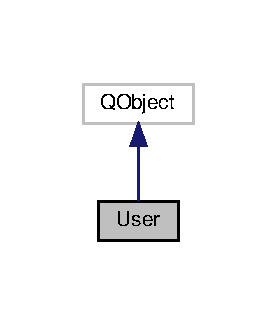
\includegraphics[width=133pt]{classUser__inherit__graph}
\end{center}
\end{figure}


Collaboration diagram for User\+:
\nopagebreak
\begin{figure}[H]
\begin{center}
\leavevmode
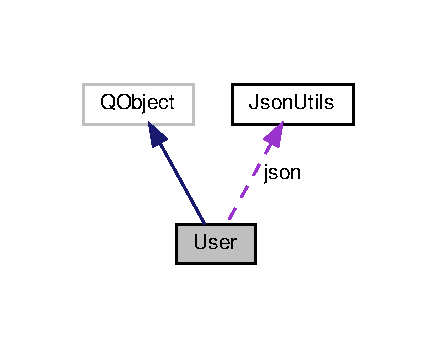
\includegraphics[width=210pt]{classUser__coll__graph}
\end{center}
\end{figure}
\subsection*{Public Member Functions}
\begin{DoxyCompactItemize}
\item 
\mbox{\Hypertarget{classUser_ae90821c4c8cc9a5a370f0ad6157adcc1}\label{classUser_ae90821c4c8cc9a5a370f0ad6157adcc1}} 
{\bfseries User} (Q\+Object $\ast$parent=nullptr)
\item 
\hyperlink{classUser_a78cce0bf7baacf9dcc0ecba524f67b87}{User} (Q\+Json\+Object user)
\item 
bool \hyperlink{classUser_a9e1fe4ac5c94a98f82ca09fa0982e029}{is\+Unique} ()
\begin{DoxyCompactList}\small\item\em \hyperlink{classUser_a9e1fe4ac5c94a98f82ca09fa0982e029}{User\+::is\+Unique}, Checks whether a \hyperlink{classUser}{User} is unique or not. \end{DoxyCompactList}\item 
bool \hyperlink{classUser_a7fff50444765760051f4ae6fb3d58e16}{is\+Valid} ()
\begin{DoxyCompactList}\small\item\em \hyperlink{classUser_a7fff50444765760051f4ae6fb3d58e16}{User\+::is\+Valid}, Checks whether \hyperlink{classUser}{User}\textquotesingle{}s input is valid. \end{DoxyCompactList}\item 
Q\+Json\+Object \hyperlink{classUser_a2edd9754d400f097b4aa88bc087ace8b}{user\+To\+Json} ()
\begin{DoxyCompactList}\small\item\em \hyperlink{classUser_a2edd9754d400f097b4aa88bc087ace8b}{User\+::user\+To\+Json}, Transforms a \hyperlink{classUser}{User} to a Q\+Json\+Object. \end{DoxyCompactList}\item 
Q\+Json\+Array \hyperlink{classUser_af14a1fba45613d9586d8951f13f9c4a0}{scores\+As\+Json\+Array} (Q\+Vector$<$ int $>$ \&scores)
\begin{DoxyCompactList}\small\item\em \hyperlink{classUser_af14a1fba45613d9586d8951f13f9c4a0}{User\+::scores\+As\+Json\+Array}, Transforms a vector of scores to Q\+Json\+Array. \end{DoxyCompactList}\item 
Q\+String \hyperlink{classUser_ac57cd256ecaaaaabc2475647902740ba}{find\+Corresponding\+Flag} ()
\begin{DoxyCompactList}\small\item\em \hyperlink{classUser_ac57cd256ecaaaaabc2475647902740ba}{User\+::find\+Corresponding\+Flag}, finds users corresponding flag from phone number. \end{DoxyCompactList}\end{DoxyCompactItemize}
\subsection*{Public Attributes}
\begin{DoxyCompactItemize}
\item 
\mbox{\Hypertarget{classUser_af691f29bfbfaecdb752ccdf762f5d037}\label{classUser_af691f29bfbfaecdb752ccdf762f5d037}} 
\hyperlink{classJsonUtils}{Json\+Utils} {\bfseries json}
\item 
\mbox{\Hypertarget{classUser_ae4202de2b7974e92a55b913d20b03833}\label{classUser_ae4202de2b7974e92a55b913d20b03833}} 
Q\+String {\bfseries username}
\item 
\mbox{\Hypertarget{classUser_ac887622f22a898c097d156ad964be846}\label{classUser_ac887622f22a898c097d156ad964be846}} 
Q\+String {\bfseries password}
\item 
\mbox{\Hypertarget{classUser_aed78465b35175ff33ab3ca3ca1ebe450}\label{classUser_aed78465b35175ff33ab3ca3ca1ebe450}} 
Q\+String {\bfseries first\+Name}
\item 
\mbox{\Hypertarget{classUser_a3a225093bbb405dab285e74e24cef7c5}\label{classUser_a3a225093bbb405dab285e74e24cef7c5}} 
Q\+String {\bfseries last\+Name}
\item 
\mbox{\Hypertarget{classUser_a7674a8234cb3ac9ad27866181c34f3a3}\label{classUser_a7674a8234cb3ac9ad27866181c34f3a3}} 
Q\+String {\bfseries dob}
\item 
\mbox{\Hypertarget{classUser_ae7cf3e04e6aba46f20af4c6802630074}\label{classUser_ae7cf3e04e6aba46f20af4c6802630074}} 
Q\+String {\bfseries gender}
\item 
\mbox{\Hypertarget{classUser_a015d9cec85964df084486386bc6bd9d4}\label{classUser_a015d9cec85964df084486386bc6bd9d4}} 
Q\+String {\bfseries phonenumber}
\item 
\mbox{\Hypertarget{classUser_a5723ab5a77c21e173453505b9af4597f}\label{classUser_a5723ab5a77c21e173453505b9af4597f}} 
Q\+Json\+Value {\bfseries profile\+Picture}
\item 
\mbox{\Hypertarget{classUser_a7f4dadaaea03ff00240d7bd3d2e8a8fd}\label{classUser_a7f4dadaaea03ff00240d7bd3d2e8a8fd}} 
int {\bfseries game1\+High\+Score} =0
\item 
\mbox{\Hypertarget{classUser_a4ad78a4dd8e01f69618b510cf5d32cea}\label{classUser_a4ad78a4dd8e01f69618b510cf5d32cea}} 
int {\bfseries game2\+High\+Score} =0
\item 
\mbox{\Hypertarget{classUser_a521511071f8d3d804f089a0c6788780a}\label{classUser_a521511071f8d3d804f089a0c6788780a}} 
Q\+Vector$<$ int $>$ {\bfseries game1\+Scores} =\{\}
\item 
\mbox{\Hypertarget{classUser_a23644b80da955e4ca44a0f74b0b4b11e}\label{classUser_a23644b80da955e4ca44a0f74b0b4b11e}} 
Q\+Vector$<$ int $>$ {\bfseries game2\+Scores} =\{\}
\end{DoxyCompactItemize}


\subsection{Constructor \& Destructor Documentation}
\mbox{\Hypertarget{classUser_a78cce0bf7baacf9dcc0ecba524f67b87}\label{classUser_a78cce0bf7baacf9dcc0ecba524f67b87}} 
\index{User@{User}!User@{User}}
\index{User@{User}!User@{User}}
\subsubsection{\texorpdfstring{User()}{User()}}
{\footnotesize\ttfamily User\+::\+User (\begin{DoxyParamCaption}\item[{Q\+Json\+Object}]{user }\end{DoxyParamCaption})\hspace{0.3cm}{\ttfamily [explicit]}}

Gets the \hyperlink{classUser}{User} from a Q\+Json\+Object \begin{DoxyReturn}{Returns}
a user from the users.\+json 
\end{DoxyReturn}


\subsection{Member Function Documentation}
\mbox{\Hypertarget{classUser_ac57cd256ecaaaaabc2475647902740ba}\label{classUser_ac57cd256ecaaaaabc2475647902740ba}} 
\index{User@{User}!find\+Corresponding\+Flag@{find\+Corresponding\+Flag}}
\index{find\+Corresponding\+Flag@{find\+Corresponding\+Flag}!User@{User}}
\subsubsection{\texorpdfstring{find\+Corresponding\+Flag()}{findCorrespondingFlag()}}
{\footnotesize\ttfamily Q\+String User\+::find\+Corresponding\+Flag (\begin{DoxyParamCaption}{ }\end{DoxyParamCaption})}



\hyperlink{classUser_ac57cd256ecaaaaabc2475647902740ba}{User\+::find\+Corresponding\+Flag}, finds users corresponding flag from phone number. 

\begin{DoxyReturn}{Returns}
encoded flag image 
\end{DoxyReturn}
\mbox{\Hypertarget{classUser_a9e1fe4ac5c94a98f82ca09fa0982e029}\label{classUser_a9e1fe4ac5c94a98f82ca09fa0982e029}} 
\index{User@{User}!is\+Unique@{is\+Unique}}
\index{is\+Unique@{is\+Unique}!User@{User}}
\subsubsection{\texorpdfstring{is\+Unique()}{isUnique()}}
{\footnotesize\ttfamily bool User\+::is\+Unique (\begin{DoxyParamCaption}{ }\end{DoxyParamCaption})}



\hyperlink{classUser_a9e1fe4ac5c94a98f82ca09fa0982e029}{User\+::is\+Unique}, Checks whether a \hyperlink{classUser}{User} is unique or not. 

\begin{DoxyReturn}{Returns}
True if unique, False otherwise. 
\end{DoxyReturn}
\mbox{\Hypertarget{classUser_a7fff50444765760051f4ae6fb3d58e16}\label{classUser_a7fff50444765760051f4ae6fb3d58e16}} 
\index{User@{User}!is\+Valid@{is\+Valid}}
\index{is\+Valid@{is\+Valid}!User@{User}}
\subsubsection{\texorpdfstring{is\+Valid()}{isValid()}}
{\footnotesize\ttfamily bool User\+::is\+Valid (\begin{DoxyParamCaption}{ }\end{DoxyParamCaption})}



\hyperlink{classUser_a7fff50444765760051f4ae6fb3d58e16}{User\+::is\+Valid}, Checks whether \hyperlink{classUser}{User}\textquotesingle{}s input is valid. 

\begin{DoxyReturn}{Returns}
true if valid, false otherwise. 
\end{DoxyReturn}
\mbox{\Hypertarget{classUser_af14a1fba45613d9586d8951f13f9c4a0}\label{classUser_af14a1fba45613d9586d8951f13f9c4a0}} 
\index{User@{User}!scores\+As\+Json\+Array@{scores\+As\+Json\+Array}}
\index{scores\+As\+Json\+Array@{scores\+As\+Json\+Array}!User@{User}}
\subsubsection{\texorpdfstring{scores\+As\+Json\+Array()}{scoresAsJsonArray()}}
{\footnotesize\ttfamily Q\+Json\+Array User\+::scores\+As\+Json\+Array (\begin{DoxyParamCaption}\item[{Q\+Vector$<$ int $>$ \&}]{scores }\end{DoxyParamCaption})}



\hyperlink{classUser_af14a1fba45613d9586d8951f13f9c4a0}{User\+::scores\+As\+Json\+Array}, Transforms a vector of scores to Q\+Json\+Array. 


\begin{DoxyParams}{Parameters}
{\em scores} & \\
\hline
\end{DoxyParams}
\begin{DoxyReturn}{Returns}
Q\+Json\+Array of scores 
\end{DoxyReturn}
\mbox{\Hypertarget{classUser_a2edd9754d400f097b4aa88bc087ace8b}\label{classUser_a2edd9754d400f097b4aa88bc087ace8b}} 
\index{User@{User}!user\+To\+Json@{user\+To\+Json}}
\index{user\+To\+Json@{user\+To\+Json}!User@{User}}
\subsubsection{\texorpdfstring{user\+To\+Json()}{userToJson()}}
{\footnotesize\ttfamily Q\+Json\+Object User\+::user\+To\+Json (\begin{DoxyParamCaption}{ }\end{DoxyParamCaption})}



\hyperlink{classUser_a2edd9754d400f097b4aa88bc087ace8b}{User\+::user\+To\+Json}, Transforms a \hyperlink{classUser}{User} to a Q\+Json\+Object. 

\begin{DoxyReturn}{Returns}
Corresponding Q\+Json\+Object 
\end{DoxyReturn}


The documentation for this class was generated from the following files\+:\begin{DoxyCompactItemize}
\item 
Accounts\+\_\+\+Framework/user.\+h\item 
Accounts\+\_\+\+Framework/user.\+cpp\end{DoxyCompactItemize}

%--- End generated contents ---

% Index
\backmatter
\newpage
\phantomsection
\clearemptydoublepage
\addcontentsline{toc}{chapter}{Index}
\printindex

\end{document}
